% !TEX encoding = IsoLatin

\documentclass[8pt,a4paper]{article}
%\documentclass[11pt,a4paper]{report}
%\documentclass[11pt,a4paper]{book}
%\documentclass[10pt, titlepage]{book} 

\usepackage[utf8]{inputenc}
\usepackage[T1]{fontenc}
\usepackage{geometry}
\usepackage{setspace}
\usepackage{amsmath, amssymb, graphicx}
\usepackage{hyperref}
\usepackage{titlesec}
\usepackage{enumitem}
\usepackage{xcolor}
%\usepackage[french]{babel}
\usepackage{tikz}
\usepackage{animate}
\usepackage{braket}
\usepackage{isotope}
\usepackage{mathrsfs}
\usepackage[acronym,shortcuts]{glossaries}
\usepackage[most]{tcolorbox}
\usepackage{array}
\usepackage{tabularx}
\usepackage{changepage}
%\usepackage{bm}
\usepackage{titlesec}
\usepackage[Glenn]{fncychap}
\usepackage{titlesec}
\usepackage{ragged2e}
\usepackage{varwidth}
\usepackage{spath3}
\usepackage{wrapfig}
\usepackage{caption}
\usepackage{enumitem}

\usetikzlibrary{animations}

%\usepackage[explicit]{titlesec}
%\usepackage{soul}
%\usepackage{lua-ul}

\usetikzlibrary{
  calc,
  positioning,
  intersections,
  decorations.pathmorphing,
  decorations.markings,
  decorations.text,
  shapes.geometric,
  arrows.meta,
  shadows,
  decorations.text,
  arrows.meta
}
\usetikzlibrary{spath3, intersections}


\titleformat{\section}{\Large\bfseries}{\thesection}{1em}{}
\titleformat{\subsection}{\large\bfseries}{\thesubsection}{1em}{}
\titleformat{\paragraph}[runin]{\bfseries}{\theparagraph}{1em}{}
\setlength{\parskip}{0.8em}
\setlength{\parindent}{0pt}

\makeatletter
\newcommand\xleftrightarrow[2][]{%
  \ext@arrow 9999{\longleftrightarrowfill@}{#1}{#2}}
\newcommand\longleftrightarrowfill@{%
  \arrowfill@\leftarrow\relbar\rightarrow}
\makeatother

\hypersetup{
  linkcolor=linkcolor, % couleur des liens internes (acronymes, toc, refs…)
  citecolor=linkcolor, % couleur des citations
  urlcolor=linkcolor   % couleur des URLs
}

\geometry{margin=1.0cm}
\setlist[itemize]{topsep=3pt,parsep=0pt,partopsep=0pt}


\newcommand{\dfonc}[1]{\mathscr{D}_{[#1]}}
%\newcommand{\operator}[1]{\hat{\bm{#1}}} % pour les operaeur vecteur
\newcommand{\operator}[1]{\hat{\boldsymbol{#1}}}

\definecolor{Prune}{RGB}{99,0,60} % l14-33 :

% --- Bois (palette principale)
\definecolor{woodNoyer}{HTML}{3A2A1F}
\definecolor{woodChene}{HTML}{4A3628}
\definecolor{woodAcajou}{HTML}{5B2C2C}

% --- Verts profonds
\definecolor{greenForet}{HTML}{0B3D2E}
\definecolor{greenSapin}{HTML}{0F4C3A}

% --- Neutres
\definecolor{grayPierre}{HTML}{4A4A4A}
\definecolor{grayBrume}{HTML}{7A7A7A}

% --- Custom colors
\definecolor{cvred}{HTML}{B71C1C}
\definecolor{headerblue}{HTML}{1565C0}
\definecolor{cvgreen}{HTML}{2E7D32}

\definecolor{titleblue}{HTML}{4a7aa4}

\definecolor{colorStitre}{RGB}{140,0,0}
\definecolor{colorSStitre}{RGB}{190,140,140}
\definecolor{colorSSStitre}{RGB}{140,140,140}
\def\colorStitre{colorStitre}
\def\colorSStitre{colorSStitre}
\def\colorSSStitre{colorSSStitre}

\definecolor{colorOne}{HTML}{443E46}
%\definecolor{colorTwo}{HTML}{F6DEB8}
\definecolor{colorTwo}{HTML}{FFFFFF}
\definecolor{colorThree}{HTML}{908CA4}
\definecolor{colorFour}{HTML}{57659E}
\definecolor{colorFive}{HTML}{C57284}
\definecolor{colorSix}{HTML}{FF5B69}
\definecolor{colorGold}{HTML}{FFD700}

% Raccourcis pour les couleurs
\def\colorOne{colorOne}
\def\colorTwo{colorTwo}
\def\colorThree{colorThree}
\def\colorFour{colorFour}
\def\colorFive{colorFive}
\def\colorSix{colorSix}
\def\colorGold{colorGold}

\makeglossaries

\newacronym{LL}{LL}{Lieb–Liniger}
\newacronym{NS}{NLS}{Nonlinear Schrödinger}
\newacronym{GP}{GP}{Gross–Pitaevskii}
\newacronym{GGE}{GGE}{Generalized Gibbs Ensemble}
\newacronym{GE}{GE}{Gibbs Ensemble}
\newacronym{BA}{BA}{Bethe Ansatz}
\newacronym{FBA}{FBA}{Fermionic Bethe Ansatz}
\newacronym{TBA}{TBA}{Thermodynamic Bethe Ansatz}
\newacronym{qBEC}{qBEC}{quasi Bose–Einstein Condensate}
\newacronym{GHD}{GHD}{Generalized Hydrodynamics}
\newacronym{LDA}{LDA}{Local Density Approximation}
\newacronym{DMD}{DMD}{Dispositif de Micromirroirs Digitaux}
\newacronym{PMO}{PMO}{Piège Magnéto-Optique}
\newacronym{DC}{DC}{Direct Current}
\newacronym{AC}{AC}{Alternating Current}
\newacronym{SYRTE}{SYRTE}{Systèmes de Référence Temps-Espace}
\newacronym{DFB}{DFB}{Distributed Feedback}
\newacronym{DBR}{DBR}{Distributed Bragg Reflector}
\newacronym{TA}{TA}{Tapered Amplifier}
\newacronym{AOM}{AOM}{Acousto-Optic Modulator}
\newacronym{PBS}{PBS}{Polarizing Beam Splitter}
\newacronym{LCF}{LCF}{Laboratoire Charles Fabry}
\newacronym{C2N}{C2N}{Centre de nanosciences et de nanotechnologies}
\newacronym{BCB}{BCB}{benzocyclobuténe}
\newacronym{SiC}{SiC}{silicon carbide}
\newacronym{Au}{Au}{aurum}
%\newacronym{AOM}{AOM}{modulateur acousto-optique}
\newacronym{CCD}{CCD}{Charge-Coupled Device}
\newacronym{TF}{TF}{Thomas-Fermi}
\newacronym{CESQ}{CESQ}{Centre européen de sciences quantiques}
\newacronym{QED}{QED}{Quantum Electrodynamics}
\newacronym{BCS}{BCS}{Bardeen–Cooper–Schrieffer}
\newacronym{YY}{YY}{Yang–Yang}
\newacronym{TG}{TG}{Tonks-Girardeau}
\newacronym{MFT}{MFT}{Macroscopic Fluctuation Theory}
\newacronym{GOE}{GOE}{Gaussian Orthogonal Ensemble}
\newacronym{GUE}{GUE}{Gaussian Unitary Ensemble}
\newacronym{RMT}{RMT}{Random Matrix Theory}
\newacronym{ABA}{ABA}{Algebraic Bethe Ansatz}

%\usepackage[french]{babel}
%\usetikzlibrary{babel}
\tikzset{
  every picture/.style={
      execute at begin picture={\shorthandoff{:;!?}}
    }
}

\tikzstyle{every picture}+=[remember picture]
\tikzstyle{na} = [shape=ellipse,inner sep=0pt]

% \newcommand{\sectiontikz}[1]{

%   \noindent
%   \begin{tikzpicture}[baseline=(title.base)]

%     \node[
%       inner sep=2pt
%     ] (title)
%     {
%       \fontsize{24}{24}\selectfont
%       \bfseries
%       #1
%     };

%     \draw[titre, line width=5pt]
%     ([xshift=-6cm]title.west) --
%     ([xshift=-0.7cm]title.west);

%     \draw[titre, line width=5pt]
%     ([xshift=0.7cm]title.east) --
%     ([xshift=6cm]title.east);

%   \end{tikzpicture}

% }

% \newcommand{\sectiontikz}[1]{
%   \vspace{-0.5cm}
%   \noindent
%   \begin{tikzpicture}

%     % Titre centré
%     \node[
%       inner sep=2pt,
%       %text width=0.7\linewidth,
%       %align=justify,
%       align=center, text width=min(0.7\linewidth,\widthof{
%         \fontsize{15}{10}\selectfont \bfseries {\Roman{section}}\ -\ #1}),
%       font=\fontsize{15}{10}\selectfont \bfseries, ] (title) at (\linewidth/2,0) {
%       {\Roman{section}}\ -\ #1 };%color = colorStitre 

%     % Ligne gauche
%     \draw[colorStitre, line width=5pt]
%     (0,0) --
%     ([xshift=-0.7cm]title.west);

%     % Ligne droite
%     \draw[colorStitre, line width=5pt]
%     ([xshift=0.7cm]title.east) --
%     (\linewidth,0);

%   \end{tikzpicture}

% }

\newcommand{\sectiontikz}[1]{
  %\vspace{-0.5cm}
  \noindent
  \begin{tikzpicture}

    \node[
      inner sep=0pt,
      %text width=0.7\linewidth,
      %align=justify,
      align=center, font=\fontsize{15}{10}\selectfont \bfseries, color = colorStitre
    ] (title) at (\linewidth/2,0) {
      \begin{varwidth}{0.7\linewidth}
        \centering
        {\Roman{section}}\ -\ #1
      \end{varwidth}
    };

    \draw[colorStitre,line width=0.3cm]
    (0,0)
    --
    ([xshift=-0.5cm]title.west);

    \draw[colorStitre,line width=0.3cm]
    ([xshift=0.5cm]title.east)
    --
    (\linewidth,0);

  \end{tikzpicture}

}

\titleformat{\section}
{\normalfont}
{}
{-1.8mm}
{\sectiontikz}
[\vspace{-1.0cm}]

%

%\titleformat{\section}{FORMAT}{LABEL}{SEP}{CODE}
%\titleformat{commande}[forme]{format}{label}{sep}{before-code}[after-code]\thesection

%\titlespacing*{\section}{0pt}{1cm}{0.7cm}

\newcommand{\subsectiontikz}[1]{
  %\vspace{-0.5cm}
  \noindent
  \begin{tikzpicture}

    \node[
      inner sep=0pt,
      %text width=0.7\linewidth,
      %align=justify,
      align=center, font=\fontsize{12}{10}\selectfont \bfseries, color = colorSStitre
    ] (title) at (\linewidth/2,0) {
      \begin{varwidth}{0.7\linewidth}
        \centering
        \thesubsection\ -\ #1
      \end{varwidth}
    };

    \draw[colorSStitre,line width=0.15cm]
    (0,0)
    --
    ([xshift=-0.3cm]title.west);

    \draw[colorSStitre,line width=0.15cm]
    ([xshift=0.3cm]title.east)
    --
    (\linewidth,0);

  \end{tikzpicture}

}

\titleformat{\subsection}
{\normalfont}
{}
{0pt}
{\subsectiontikz}
[\vspace{-1.0cm}]

\newcommand{\subsubsectiontikz}[1]{
  %\vspace{-0.5cm}
  \noindent
  \begin{tikzpicture}

    \node[
      inner sep=0pt,
      %text width=0.7\linewidth,
      %align=justify,
      align=center, font=\fontsize{10}{10}\selectfont \bfseries, color =
      colorSSStitre ] (title) at (\linewidth/2,0) {
      \begin{varwidth}{0.7\linewidth}
        \centering
        \thesubsubsection\ -\ #1
      \end{varwidth}
    };

    \draw[colorSSStitre,line width=0.10cm]
    (0,0)
    --
    ([xshift=-0.2cm]title.west);

    \draw[colorSSStitre,line width=0.10cm]
    ([xshift=0.2cm]title.east)
    --
    (\linewidth,0);

  \end{tikzpicture}

}

\titleformat{\subsubsection}
{\normalfont}
{}
{0pt}
{\subsubsectiontikz}
[\vspace{-1.0cm}]

%\newcommand{\ptFleche}[2]{		% Déclaration d'une extrémité de flèche
%    \shorthandoff{:;!?}% <- désactive les shorthands
%    \tikz[baseline=(#1.base)]\node[na](#1){#2};
%  }

\newcommand{\ptFleche}[2]{%
  \tikz[baseline=(#1.base)]{
    \shorthandoff{:;!?}
    \node[na](#1){#2};
  }%
}

\newcommand{\Fleche}[5][thick]{%
  \begin{tikzpicture}[overlay]
    \path[->,#1](#2) edge [out=#4, in=#5] (#3);
  \end{tikzpicture}
}

% --- Commande FlecheEllipse ---
% #1 = nœud source (nom)
% #2 = angle sortie du nœud source
% #3 = angle entrée du nœud cible
% #4 = décalage dx, dy sous forme (dx,dy) en cm
% #5 = couleur ellipses et flèche
% #6 = texte du nœud cible B
\newcommand{\FlecheEllipseo}[6]{%
  \begin{tikzpicture}[overlay, remember picture]
    % Coordonnées source
    \path let \p1 = (#1) in
    coordinate (Acoord) at (\x1,\y1);

    % Coordonnées cible
    \pgfmathsetmacro{\dx}{#4}
    \pgfmathsetmacro{\dy}{#5} % ici on sépare les deux pour le calcul

    \coordinate (B) at ([shift={(#4)}]#1);

    % Nœud A entouré d'ellipse
    \node[draw,#5,ellipse,inner sep=2pt] (#1-node) at (#1) {#1};
    % Nœud B entouré d'ellipse
    \node[draw,#5,ellipse,inner sep=2pt] (B-node) at (B) {#6};
    % Flèche de A vers B
    \draw[->,#5,thick] (#1-node) edge [out=#2,in=#3] (B-node);
  \end{tikzpicture}%
}

% --- Commande FlecheEllipse finale ---
% #1 = nom du nœud source (A)
% #2 = angle sortie du nœud source
% #3 = angle entrée du nœud cible
% #4 = décalage horizontal dx (en cm)
% #5 = décalage vertical dy (en cm)
% #6 = couleur ellipses et flèche
% #7 = contenu du nœud B (texte, formule, TikZ, etc.)
\newcommand{\FlecheEllipse}[7]{%
  \begin{tikzpicture}[overlay]
    % --- Nœud source A ---
    \node[draw,#6,ellipse,inner sep=2pt](#1){};

    % --- Nœud cible B ---
    \coordinate (B) at ($(#1) + (#4cm,#5cm)$);
    \node[draw,#6,ellipse,inner sep=2pt] (B-node) at (B) {#7};

    % --- Flèche de A vers B ---
    \draw[->,#6,thick] (#1) edge [out=#2,in=#3] (B-node);
  \end{tikzpicture}%
}

\renewcommand{\arraystretch}{0.2}

% Custom commands for events
\newcommand{\cvdegree}[6]{%
  \textbf{#1} & \textbf{#2} -- #3 \\
  & \textit{#4} {\color{headerblue}} \\
  & #5 \\[0.6em]
}

\newcommand{\cvevent}[6]{%
  \textbf{#1} & \textbf{#2} -- #3 \\
  & \textit{#4} {\color{cvred}} \\
  & #5 \\[0.6em]
}

\tcbuselibrary{skins}

\NewTotalTColorBox[auto counter]{\Example}{ +m +m }{
  enhanced,
  notitle,
  colback=white,
  colbacklower=white,
  frame hidden,
  boxrule=0pt,
  bicolor,
  sharp corners,
  %borderline west={4pt}{0pt}{greenForet},
  left=3mm, fontupper=\sffamily, overlay={% espace pour le texte vertical
      % Bande verticale
      \fill[greenForet]
      (frame.south west) rectangle
      ([xshift=4pt]frame.north west);

      % Texte vertical
      \node[
        rotate=90,
        anchor=south,
        font=\sffamily\bfseries,
        text=greenForet
      ] at ([xshift=2pt]frame.west) {#1};

      % Texte vertical centré
      \node[
        rotate=90,
        anchor=center,
        font=\sffamily\bfseries,
        text=white
      ] at ([xshift=2pt]frame.west |- frame.center) {Example};
    }
}{
  \textcolor{greenForet}{
    \sffamily\textbf{Exemple~: #1}\\
  }
  #2
}

\newcommand{\EncadreDeux}[4]{%
  \begin{tcolorbox}[
      enhanced,
      notitle,
      colback=white,
      colbacklower=white,
      frame hidden,
      boxrule=0pt,
      sharp corners,
      borderline west={4pt}{0pt}{#3},
      left=7mm,
      fontupper=\sffamily,
      overlay={%
          % Bande verticale
          \fill[#3]
          (frame.south west) rectangle
          ([xshift=4pt]frame.north west);

          \node[
            rotate=90,
            anchor=south,
            font=\sffamily\bfseries,
            text=#3
          ] at ([xshift=2pt]frame.west) {#2};

          % Texte vertical (titre)
          \node[
            rotate=90,
            anchor=center,
            font=\sffamily\bfseries\small,
            text=white
          ] at ([xshift=2pt]frame.west |- frame.center)
          {#1};

        }
    ]
    % contenu
    %\textcolor{#3}{\sffamily\textbf{#1}}\\
    #4
  \end{tcolorbox}
}

\NewTotalTColorBox[auto counter]{\Information}{+m}{
  enhanced,
  notitle,
  colback=white,
  colbacklower=white,
  frame hidden,
  boxrule=0pt,
  sharp corners,
  left=3mm,
  fontupper=\sffamily,
  overlay={
      % Bande verticale
      \fill[grayPierre]
      (frame.south west) rectangle
      ([xshift=4pt]frame.north west);

      % Texte vertical
      % \node[
      %     rotate=90,
      %     anchor=south,
      %     font=\sffamily\bfseries,
      %     text=grayPierre
      % ] at ([xshift=2pt]frame.west) {Information};

      % Texte vertical centré
      \node[
        rotate=90,
        anchor=center,
        font=\sffamily\bfseries,
        text=white
      ] at ([xshift=2pt]frame.west |- frame.center) {Information};
    },
}{
  #1
}

\NewTotalTColorBox[auto counter]{\ARetenir}{+m}{
  enhanced,
  notitle,
  colback=white,
  colbacklower=white,
  frame hidden,
  boxrule=0pt,
  bicolor,
  sharp corners,
  %borderline west={4pt}{0pt}{woodChene},
  left=3mm, fontupper=\sffamily, overlay={
      % Bande verticale
      \fill[woodChene]
      (frame.south west) rectangle
      ([xshift=4pt]frame.north west);

      % Texte vertical
      % \node[
      %     rotate=90,
      %     anchor=south,
      %     font=\sffamily\bfseries,
      %     text=woodChene
      % ] at ([xshift=2pt]frame.west) {À Retenir};

      % Texte vertical centré
      \node[
        rotate=90,
        anchor=center,
        font=\sffamily\bfseries,
        text=white
      ] at ([xshift=2pt]frame.west |- frame.center) {À Retenir};
    },
}{
  % \textcolor{woodChene}{
  %     \sffamily\textbf{À retenir~: #1}
  % }
  #1
}

% \newcommand{\EncadreUn}[3]{

% \NewTotalTColorBox[auto counter]{\ARetenir}{+m}{
%   enhanced,
%   notitle,
%   colback=white,
%   colbacklower=white,
%   frame hidden,
%   boxrule=0pt,
%   bicolor,
%   sharp corners,
%   borderline west={4pt}{0pt}{#3},
%   left=3mm, fontupper=\sffamily, overlay={
%       % Bande verticale
%       \fill[#3]
%       (frame.south west) rectangle
%       ([xshift=4pt]frame.north west);

%       % Texte vertical centré
%       \node[
%         rotate=90,
%         anchor=center,
%         font=\sffamily\bfseries,
%         text=white
%       ] at ([xshift=2pt]frame.west |- frame.center) {#1};
%     },
% }{
%   #2
% }

% }

\newcommand{\EncadreUn}[3]{%
  \begin{tcolorbox}[
      enhanced,
      notitle,
      colback=white,
      colbacklower=white,
      frame hidden,
      boxrule=0pt,
      sharp corners,
      borderline west={4pt}{0pt}{#2},
      left=6mm,
      fontupper=\sffamily,
      overlay={
          % Bande verticale
          \fill[#2]
          (frame.south west) rectangle
          ([xshift=4pt]frame.north west);

          % Texte vertical
          \node[
            rotate=90,
            anchor=center,
            font=\sffamily\bfseries\small,
            text=white
          ] at ([xshift=2pt]frame.west |- frame.center)
          {#1};
        }
    ]
    #3
  \end{tcolorbox}
}

\NewTotalTColorBox[auto counter]{\Rappel}{+m}{
  enhanced,
  notitle,
  colback=white,
  colbacklower=white,
  frame hidden,
  boxrule=0pt,
  bicolor,
  sharp corners,
  %borderline west={4pt}{0pt}{woodNoyer},
  left=3mm, fontupper=\sffamily, overlay={
      % Bande verticale
      \fill[woodNoyer]
      (frame.south west) rectangle
      ([xshift=4pt]frame.north west);

      % Texte vertical
      % \node[
      %     rotate=90,
      %     anchor=south,
      %     font=\sffamily\bfseries,
      %     text=woodNoyer
      % ] at ([xshift=2pt]frame.west) {Rappel};

      % Texte vertical centré
      \node[
        rotate=90,
        anchor=center,
        font=\sffamily\bfseries,
        text=white
      ] at ([xshift=2pt]frame.west |- frame.center) {Rappel};
    },
}{
  % \textcolor{woodNoyer}{
  %     \sffamily\textbf{Rappel~: #1}
  % }
  #1
}

\NewTotalTColorBox[auto counter]{\Resume}{+m}{
  enhanced,
  notitle,
  colback=white,
  colbacklower=white,
  frame hidden,
  boxrule=0pt,
  bicolor,
  sharp corners,
  %borderline west={4pt}{0pt}{woodAcajou},
  left=3mm, fontupper=\sffamily, overlay={
      % Bande verticale
      \fill[woodAcajou]
      (frame.south west) rectangle
      ([xshift=4pt]frame.north west);

      % Texte vertical
      % \node[
      %     rotate=90,
      %     anchor=south,
      %     font=\sffamily\bfseries,
      %     text=woodAcajou
      % ] at ([xshift=2pt]frame.west) {Conclusion};

      % Texte vertical centré
      \node[
        rotate=90,
        anchor=center,
        font=\sffamily\bfseries,
        text=white
      ] at ([xshift=2pt]frame.west |- frame.center) {Conclusion};
    },
}{
  % \textcolor{woodAcajou}{
  %     \sffamily\textbf{Conclusion~: #1}
  % }
  #1
}

% Définition de la fonction pour générer la grille
% \newcommand{\drawgrid}[4]{

%   \begin{scope}[opacity = 0.2]

%     % Paramètres : #1=xmin, #2=xmax, #3=ymin, #4=ymax

%     % Grille principale en cm
%     \draw[very thin, gray] (#1,#3) grid (#2,#4); % Grille de base (1 cm)

%     \draw[very thin, gray] (#1,#3) grid[step=0.1] (#2,#4);

%     \draw[thin, black] (#1,#3) edge[thick,line width=0.8ex,->,>=Stealth ] (#2,#3);

%     \foreach \x in {#1,..., #2} {
%         \draw[shift={(\x, #3)}] (0,-0.1) edge[line width=0.8ex] node[pos = -1 , below] {\x} (0,0.1); % Lignes verticales en mm
%       }

%     \draw[thin, black] (#1,#3)edge[thick,line width=0.8ex,->,>=Stealth ] (#1,#4);

%     \foreach \y in {#3,..., #4} {
%         \draw[shift={(#1, \y)}] (-0.1 , 0 ) edge[line width=0.8ex] node[pos = -1 , left ] {\y} (0.1 , 0); % Lignes verticales en mm
%       }

%   \end{scope}

% }

% Définition de la fonction pour générer la grille
\newcommand{\drawgrid}[4]{

  % #1 xmin
  % #2 xmax
  % #3 ymin
  % #4 ymax

  \begin{scope}[opacity=0.2]

    % Taille des axes
    \pgfmathsetmacro{\dx}{#2-#1}
    \pgfmathsetmacro{\dy}{#4-#3}

    % ======================
    % Grille principale
    % ======================

    \draw[very thin, gray]
    (#1,#3) grid (#2,#4);

    \draw[very thin, gray]
    (#1,#3) grid[step=0.1] (#2,#4);

    % ======================
    % Grille fine conditionnelle
    % ======================

    \ifdim \dx pt < 0.5pt

      \draw[very thin, gray , line width=0.01mm ]
      (#1,#3) grid[step=0.01] (#2,#4);

    \fi

    \ifdim \dy pt < 0.5pt

      \draw[very thin, gray , line width=0.01mm]
      (#1,#3) grid[step=0.01] (#2,#4);

    \fi

    % ======================
    % Axe x
    % ======================

    \draw[thick,line width=0.8ex,->,>=Stealth]
    (#1,#3) -- (#2,#3);

    \foreach \x in {#1,...,#2} {

        \draw[shift={(\x,#3)}]
        (0,-0.1) --
        (0,0.1)

        node[pos=-1,below] {\x};

      }

    % ======================
    % Axe y
    % ======================

    \draw[thick,line width=0.8ex,->,>=Stealth]
    (#1,#3) -- (#1,#4);

    \foreach \y in {#3,...,#4} {

        \draw[shift={(#1,\y)}]
        (-0.1,0) --
        (0.1,0)

        node[pos=-1,left] {\y};

      }

  \end{scope}

}

% \title{%
% Étude de la dynamique hors équilibre\\
% des gaz de bosons unidimensionnels
% }

% \author{%
% Guillaume Thémèze\\
% <guillaume.themeze@gmail.fr>
% }

% \date{%
% Thèse de doctorat\\
% Université Paris-Saclay\\
% Soutenue le \today
% }

% \date{\today}

\begin{document}

\begin{center}
    {\LARGE \textbf{Mise en perspective didactique d’un dossier de recherche}}\\[1em]
    \textbf{Guillaume THÉMÈZE}\\[0.5em]
    Concours externe spécial de l’agrégation de physique-chimie, option physique, session 2026
\end{center}

\vspace{-0.0cm}

\section{Formations et expériences}

\subsection{Formation académique}

\begin{tabular}{r p{0.85\textwidth}}

    \cvdegree{2022--2025 :}{Thèse de Doctorat en physique quantique}{à \textit{l'Université de Paris-Saclay /
            Institut d’Optique Graduate School (IOGS) / Laboratoire Charles Fabry (LCF) ,} intitulée \textit{Étude de la dynamique hors équilibre de gaz bosoniques unidimensionnels} sous la direction d'Isabelle Bouchoule.}{}{}{}                                 %\\   [0.1em]

    \cvdegree{2021--2022 :}{Master 2 Quantum, Light, Matter, Nanoscience (QLMN)}{Master recherche,
        \textit{IOGS / Université Paris-Saclay .} Spécialisation en physique quantique, optique, nanosciences et matière condensée.}{}{}{}                                                             %\\   [0.1em]

    \cvdegree{2020--2021 :}{Master 2 Métiers de l’Enseignement, de l’Éducation et de la Formation (MEEF) + Préparation à l’Agrégation, École Normale Supérieure (ENS) Ulm \& Université  Paris-Saclay}{Physique-Chimie option Physique}{}{}{} %\\   [0.1em]

    \cvdegree{2018--2021 :}{Magistère de physique fondamentale}{(L3–M2)
        \textit{Université Paris-Sud .}Formation approfondie en physique théorique et expérimentale, stages de recherche, enseignements complémentaires (langues, informatique, gestion).}{}{}{}                                                                    %\\   [0.1em]

    \cvdegree{2015--2018 :}{Classe Préparatoire aux Grandes Écoles}{ (CPGE), filière MPSI/MP,
        \textit{Lycée Leconte de Lisle (Réunion) \& Lycée La Martinière Momplaisire (Lyon)}}{}{}{}
\end{tabular}

\vspace{-0.5cm}
\subsection{Expérience de recherche}

\begin{tabular}{r p{0.85\textwidth}}

    %\cvdegree{2022--2025 :}{Doctorat – Activité de recherche}{\textit{IOGS / LCF .}Étude des gaz quantiques hors équilibre : approche combinée théorique, numérique et expérimentale. Développement de modèles, simulations et mesures locales de densité (cf. [1,2,3]).}{}{}{} %\\   [0.1em]

    \cvdegree{2022 :}{Stage de Master 2}{\textit{IOGS / LCF .} Dynamique d’un gaz bosonique unidimensionnel : modélisation théorique, simulations et mesures expérimentales.}{}{}{}            %\\   [0.1em]

    \cvdegree{2020 :}{Stage de Master 1}{\textit{Université Paris-Saclay .} Expansion maximale des trous noirs de Schwarzschild \& de Kerr. Analyse théorique et simulations.}{}{}{}               %\\   [0.1em]

    \cvdegree{2019 :}{Stage de Licence 3}{\textit{École Polytechnique (l’X) / Laboratoire de Physique des Plasmas (LPP)} modélisation théorique et numérique.}{}{}{}                            %\\   [0.1em]

\end{tabular}

\vspace{-0.5cm}
\subsection{Expérience d’enseignement}

\begin{tabular}{r p{0.85\textwidth}}

    \cvdegree{2023--2026 :}{Chargé d’enseignement (TD/TP)}{
        \textit{IOGS (SupOptique, Institut Polytechnique de Paris) \& Polytech Paris-Saclay}
        Travaux dirigés en mécanique quantique et traitement du signal (L3).
        Travaux pratiques en physique des lasers (M1/M2).
        Plus de 200 heures d’enseignement.}{}{}{}                                                                               %\\   [0.1em]

    \cvdegree{2021--2023 :}{Soutien scolaire}{\textit{Association Effiscience}
        Cours particuliers de Mathématique et de physique pour des classes de 5 élèves, niveau collège et lycée.}{}{}{}        %\\   [0.1em]

    \cvdegree{2019 :}{Stage d’observation pédagogique}{\textit{Lycée de l'Essouriau (91940) Les Ulis}
        Observation et participation à des cours de physique-chimie.
        Découverte des méthodes d’enseignement en lycée.}{}{}{}                                                                 %\\   [0.1em]

    \cvdegree{2019 :}{Colles de Mathématique et de Physique}{\textit{en MP, Lycée La Martinière Momplaisire (Lyon)}}{}{}{} %\\   [0.1em]

\end{tabular}

% \paragraph{Orientation scientifique et pédagogique}
% Mon parcours, à la croisée de la \textbf{physique fondamentale}, de la
% \textbf{modelisation numérique} et de la \textbf{transmission du savoir}, m’a
% conduit à développer une double compétence en \textit{recherche théorique} et
% en \textit{enseignement expérimental}. L’intégration de la démarche
% scientifique dans un cadre pédagogique constitue le fil conducteur de mes
% expériences.

% \subsection{Expériences de recherche}
% \begin{itemize}
%     \item Mise en place et analyse de modèles de dynamique quantique hors équilibre.
%     \item Développement d’outils de simulation (Python / Julia / HPC) et d’algorithmes
%           d’optimisation.
%     \item Collaboration interdisciplinaire (données expérimentales, modélisation
%           analytique).
% \end{itemize}

% \paragraph{Orientation scientifique et pédagogique}

% Ma formation en physique fondamentale, prolongée par une thèse en physique
% quantique au sein de l’Institut d’Optique Graduate School et du Laboratoire
% Charles Fabry, m’a permis de développer une approche articulant
% \textbf{modélisation théorique}, \textbf{analyse numérique} et
% \textbf{expérimentale}.

% Mes travaux de recherche portent principalement sur l’étude des systèmes
% quantiques hors équilibre et des gaz bosoniques unidimensionnels, à l’interface
% entre mécanique quantique, physique statistique et simulation numérique. Cette
% activité s’est accompagnée du développement d’outils scientifiques en
% \texttt{Python}, \texttt{Julia} et \texttt{Bash}, ainsi que de la production de
% supports scientifiques et pédagogiques sous \LaTeX{} et TikZ.

% Parallèlement, mes expériences d’enseignement en travaux dirigés et pratiques
% auprès d’étudiants de licence, master et école d’ingénieur ont renforcé mon
% intérêt pour la transmission des concepts fondamentaux de la physique. Je porte
% une attention particulière à l’articulation entre rigueur théorique,
% visualisation des phénomènes physiques et mise en activité des étudiants.

% L’ensemble de ce parcours s’inscrit dans une volonté de relier démarche de
% recherche, outils numériques et pédagogie scientifique au service de
% l’enseignement de la physique.

% \subsection{Activités scientifiques et compétences développées}

% \begin{itemize}

%     \item Étude théorique  numérique et expérimental de la dynamique hors équilibre de systèmes quantiques fortement corrélés.

%     \item Développement de modèles analytiques et simulations numériques appliqués aux
%           gaz quantiques unidimensionnels.

%     \item Exploitation et interprétation de données expérimentales en interaction avec
%           des travaux de physique atomique.

%     \item Développement d’outils scientifiques et numériques (\texttt{Python},
%           \texttt{Julia}, \texttt{Bash}) pour la simulation, automatisation de taches,
%           l’analyse de données et l’automatisation de traitements.

%     \item Conception de documents scientifiques et pédagogiques sous \LaTeX{}, TikZ,
%           HTML/CSS/JavaScript et gestion de projets via GitHub.

%     \item Expérience de transmission des savoirs en physique théorique, traitement du
%           signal et physique expérimentale auprès d’étudiants de licence, master et école
%           d’ingénieur.

%     \item Travail collaboratif dans un environnement interdisciplinaire associant
%           théorie, simulation numérique et expérience.

% \end{itemize}

\paragraph{Orientation scientifique et pédagogique}

Ma formation en physique fondamentale, prolongée par une thèse en physique
quantique, m’a conduit à développer des compétences en \textbf{modélisation
    théorique}, \textbf{simulation et analyse numérique} ainsi qu’en
\textbf{physique expérimentale}. Mes travaux de recherche, menés dans un
environnement interdisciplinaire associant théorie, simulation numérique et
expérience, m’ont également amené à vulgariser et transmettre des concepts
physiques abstraits. Parallèlement à mes activités de recherche, j’ai développé
une expérience d’enseignement auprès d’étudiants de lycée, de licence, de
master et d’école d’ingénieur, ainsi que des outils scientifiques et
pédagogiques (\texttt{Python}, \texttt{Julia}, \LaTeX{}, \texttt{TikZ},
\texttt{HTML}/\texttt{CSS}/\texttt{JavaScript}/\texttt{JSON}, \texttt{Bash},
\texttt{GitHub}) destinés à la simulation, à la visualisation et à la
transmission des concepts de physique. Mes expériences m’ont conduit à accorder
une attention particulière à l’articulation entre rigueur scientifique, outils
numériques et pédagogie.

% \section{Enseignement}

% \paragraph{Encadrements universitaires}
% \begin{itemize}
%     \item TD de Mécanique quantique et traitement du signal (niveau L3) à l'Institut
%           d'optique.
%     \item TP de Physique des lasers (niveau M1–M2) à Polytech.
% \end{itemize}
% Ces expériences m’ont permis d’adapter des contenus académiques abstraits à un public hétérogène, en privilégiant des approches visuelles et numériques.

% \paragraph{Pédagogie et réflexivité}
% Mon objectif est de développer chez l’élève une compréhension \textit{active} :
% à partir d’un phénomène observé ou simulé, formuler un modèle, identifier ses
% limites, puis le confronter aux données. La clarification progressive des
% hypothèses devient ainsi l’outil le plus puissant pour enseigner la rigueur
% scientifique.

% \section{Enseignement}

% \paragraph{Encadrements universitaires}
% \begin{itemize}
%     \item TD de Mécanique quantique et traitement du signal (niveau L3) à l'Institut
%           d'optique.
%     \item TP de Physique des lasers (niveau M1–M2) à Polytech.
% \end{itemize}

% Ces expériences m’ont permis d’adapter des contenus académiques abstraits à un
% public hétérogène, en privilégiant des approches visuelles et numériques, ainsi
% qu’un lien constant entre théorie et expérience.

% \paragraph{Interventions en lycée}
% J’ai également eu l’occasion d’intervenir ponctuellement en lycée, notamment
% sous forme de présentations ciblées (10 à 15 minutes), visant à introduire des
% notions de physique moderne de manière accessible. Ces interventions montrent
% que, même à ce niveau, il est possible d’aborder des concepts avancés en
% s’appuyant sur des analogies, des expériences simples et des supports visuels.

% \paragraph{Pédagogie et réflexivité}

% Mon objectif est de développer chez l’étudiant une compréhension
% \textit{active} : à partir d’un phénomène observé ou simulé, formuler un
% modèle, identifier ses hypothèses, puis en discuter les limites. La
% clarification progressive de ces hypothèses constitue, selon moi, un levier
% central pour enseigner la rigueur scientifique.

% Dans mes enseignements, je commence généralement chaque séance par une courte
% introduction (5 à 15 minutes) présentant les notions essentielles. En amont, je
% demande aux étudiants de préparer le TD et de m’envoyer leurs questions, ce qui
% me permet d’adapter la séance à leurs difficultés réelles. Je prépare également
% une correction détaillée incluant le cours, ainsi que des questions types
% issues de mon expérience d’étudiant ou rencontrées lors de la préparation des
% séances.

% Je m’appuie fortement sur des supports rédigés en \LaTeX{}, intégrant des
% schémas et animations (notamment avec TikZ), que j’enrichis d’année en année.
% Ces documents me servent de fil conducteur et me permettent, en séance, de me
% concentrer sur l’essentiel sans dépendre d’un support écrit. Bien que
% j’encourage les étudiants à prendre des notes manuscrites, je mets à leur
% disposition ces documents complets afin de ne pas pénaliser ceux qui
% rencontrent des difficultés à suivre simultanément la compréhension et la prise
% de notes. Cette attention est particulièrement importante pour des étudiants
% présentant des troubles de type dyslexie.

% Je veille également à favoriser l’interactivité : je sollicite régulièrement
% les étudiants, les invite à venir au tableau et à proposer des démarches de
% résolution. Conscient de l’appréhension que cela peut susciter, j’essaie
% d’instaurer un climat de confiance et de bienveillance, afin que chacun puisse
% participer. Cette dynamique collective est essentielle pour maintenir
% l’engagement et permettre une appropriation réelle des concepts.

% Enfin, le fait de préparer soigneusement les séances en amont me permet de
% garder une vision claire du fil directeur, d'avoir les questions en tète, tout
% en conservant une certaine spontanéité dans la résolution des problèmes. Cette
% approche renforce, selon moi, la crédibilité de l’enseignant et favorise
% l’adhésion des étudiants.

\newpage

\section{Enseignement}

\EncadreDeux
{}{{\bf \textsf{Expériences d’enseignement}}}{woodChene}{
    \paragraph{Expériences d’enseignement}

    Au cours de mon parcours, j’ai eu l’occasion d’enseigner à différents niveaux,
    du lycée au master, dans des contextes variés mêlant soutien pédagogique,
    travaux dirigés et travaux pratiques expérimentaux.

    En lycée, dans le cadre de cours particuliers en mathématiques et physique,
    j’ai accompagné des élèves sur l’ensemble du programme du secondaire, avec une
    attention particulière portée à la compréhension des notions fondamentales et à
    la méthodologie de résolution de problèmes.

    J’ai également réalisé des colles de mathématiques et de physique en classe
    préparatoire MP au lycée La Martinière Monplaisir, principalement dans le cadre
    des révisions précédant les épreuves orales des concours. Ces séances m’ont
    amené à travailler sur une large partie du programme de physique et de
    mathématiques de CPGE, tout en développant une approche orale et interactive de
    l’enseignement.

    À l’Institut d’Optique Graduate School, j’ai assuré des Travaux dirigés de mécanique
    quantique et de traitement du signal en L3. Les enseignements de mécanique
    quantique portaient notamment sur l’évolution d’un paquet d’onde libre,
    l’inégalité d’Heisenberg, les opérateurs et mesures, les oscillations de Rabi
    ou encore les états quasi-classiques. En traitement du signal, les séances
    abordaient les signaux aléatoires, les bruits, le filtrage adapté, le filtrage
    de Wiener, la détection et des notions de théorie de l’information.

    J’ai également encadré des Trauvaux pratiques de physique des lasers en M1/M2 à
    Polytech Paris-Saclay, portant sur l’étude expérimentale de différents types de
    lasers et de phénomènes optiques tels que les pinces optiques ou l’effet Raman.
}

\vspace{-0.0cm}

\EncadreDeux
{}{{\bf \textsf{Approche pédagogique}}}{woodChene}{
    \paragraph{Approche pédagogique}

    Dans mes enseignements, j’accorde une importance particulière aux liens entre
    les différents domaines de la physique et des mathématiques. J’essaie de
    montrer aux étudiants que de nombreux outils qu’ils découvrent dans des cadres
    différents reposent sur des structures communes. Par exemple, lors des
    enseignements de mécanique quantique, je fais régulièrement le lien entre les
    opérateurs hermitiens et le théorème spectral étudié en algèbre linéaire, ou
    encore entre l’inégalité d’Heisenberg et l’inégalité de Cauchy-Schwarz. Mon
    objectif est de leur montrer qu’ils possèdent déjà une grande partie des outils
    nécessaires, et que l’enjeu consiste souvent à apprendre à relier et
    généraliser ces concepts.

    Je commence généralement les séances par une courte introduction permettant de
    replacer les notions dans un cadre plus large et de rappeler les idées
    essentielles déjà rencontrées dans d’autres contextes. Cette approche vise à
    donner du sens aux outils mathématiques et physiques, tout en favorisant une
    compréhension plus unifiée des concepts.

    Je prépare également des supports détaillés rédigés sous \LaTeX{}, intégrant
    des schémas et animations réalisés avec TikZ, que je mets à disposition des
    étudiants afin d’accompagner la compréhension des notions abordées. Ces
    documents constituent un support pédagogique que j’enrichis progressivement au
    fil des enseignements (exemple
    \url{https://themeze.github.io/portfolio_recherche_2/physics/faculty/themeze/documents/index.html}
    / Enseignement / Mecanique quantique L3). }

% \section{Activités pédagogiques}

% \subsection{Activité 1 : Interférences quantiques simulées}
% \textbf{Niveau : Terminale Spécialité — Thèmes : Ondes et signaux.}

% Objectif : modéliser une double fente électronique sous Python et visualiser le
% rôle de la probabilité d’interférence.

% \begin{itemize}
%     \item \textit{Compétences mobilisées :} traitement du signal, lien onde-particule.
%     \item \textit{Apports :} la simulation numérique sert de médiation entre expérience de pensée et modèle probabiliste.
% \end{itemize}

% \subsection{Activité 2 : Python et loi de Planck}
% \textbf{Niveau : Première / CPGE — Thèmes : Rayonnement du corps noir, quantification de l’énergie.}
% \\À partir de données expérimentales simulées, les étudiants déterminent la température d’une étoile par ajustement numérique et observent que la loi empirique conduit naturellement à la quantification.

% \paragraph{Lien didactique}
% Ces activités intègrent la \textit{programmation scientifique} dans la démarche
% d’investigation : le calcul devient un outil de compréhension physique, non un
% simple exercice algorithmique.

\section{Travaux de recherche}

% L'étude des gaz quantiques unidimensionnels offre un cadre modèle pour explorer
% les phénomènes hors équilibre et les transitions entre régimes intégrables et
% chaotiques.

Les gaz quantiques unidimensionnels occupent une place singulière en physique
des systèmes à N corps, en constituant un véritable système modèle, analogue
aux drosophiles en biologie : suffisamment simples pour être étudiés en détail,
mais suffisamment riches pour révéler des comportements génériques de la
physique des systèmes complexes. Ils permettent d’explorer, dans un cadre
contrôlé, l’émergence de phénomènes collectifs issus de l’interaction entre
particules.

Ce système fondamental se situe à l’interface de plusieurs domaines de la
physique moderne, allant de la physique analytique et de la physique
non-linéaire à la physique statistique, ainsi qu’à la thermodynamique et à
l’hydrodynamique. Cette diversité en fait un objet privilégié pour l’étude des
systèmes fortement corrélés.

Dans ce cadre, les gaz quantiques unidimensionnels constituent un modèle
théorique particulièrement adapté à l’étude des phénomènes hors équilibre,
ainsi qu’à la compréhension des transitions entre régimes intégrables et
dynamiques chaotiques.

\vspace{-0.5cm}
\subsection{Pourquoi étudier un système unidimensionnel ? Un exemple simple : les sphères dures}

À la lecture du titre de mon mémoire de thèse, \emph{\textbf{Étude de la dynamique hors équilibre des gaz de bosons unidimensionnels}}, il est légitime de se demander pourquoi s’intéresser à des systèmes unidimensionnels, apparemment éloignés de notre réalité tridimensionnelle. L’objectif de cette introduction est d’illustrer, à travers un exemple classique, l’intérêt fondamental des systèmes de basse dimension : le modèle des \emph{sphères dures}\footnote{Voir par exemple le cours en ligne très pédagogique de Jérôme Dubail au Collège de France :
    \url{https://www.youtube.com/watch?v=t53C5hoXiw4}.}.

\subsubsection{Les sphères dures en deux dimensions}

Considérons un ensemble de particules sphériques identiques se déplaçant
librement dans un espace bidimensionnel muni de conditions aux limites
périodiques\footnote{Les conditions aux limites périodiques signifient que
    lorsqu’une particule quitte un côté du domaine, elle réapparaît instantanément
    du côté opposé avec la même vitesse. Elles permettent de simuler un système
    homogène et de taille infinie en éliminant les effets de bord.}. Les particules
n’interagissent qu’au moment des collisions élastiques.

\smallskip

Les sphères sont initialement réparties aléatoirement et immobiles. À l’instant
initial, une impulsion est appliquée à une seule particule
(figure~\ref{fig:hard_spheres_2D_animation}a), plaçant le système dans un état
fortement hors équilibre : toute l’énergie cinétique est alors concentrée dans
un unique degré de liberté, très loin de la distribution d’équilibre de
Maxwell--Boltzmann.

\smallskip

Au cours du temps, les collisions redistribuent progressivement l’énergie et
l’impulsion entre les particules. Après un temps suffisamment long, le système
atteint un état d’équilibre thermodynamique caractérisé par une distribution
des vitesses de Maxwell--Boltzmann
(figure~\ref{fig:hard_spheres_2D_animation}c). Ce processus spontané
d’évolution vers l’équilibre est appelé \emph{thermalisation}.

\smallskip

Un aspect essentiel est que le système \emph{oublie} progressivement les
détails microscopiques de son état initial. À grande échelle, sa dynamique est
entièrement décrite par quelques champs hydrodynamiques conservés : la
\textbf{densité de particules $n$}, la \textbf{densité d’impulsion $p$} et la
\textbf{densité d’énergie $e$}.

Cette émergence d’une description macroscopique universelle, indépendante des
détails microscopiques, est au cœur de la physique statistique.

\smallskip

On dit alors que le système est \emph{ergodique} ou \emph{chaotique} : au cours
du temps, il explore efficacement son espace des phases, ce qui permet la
thermalisation et l’apparition d’un comportement universel à grande échelle.

\begin{figure}[h]
    \centering
    \begin{tikzpicture}
        %\begin{scope}[transform canvas={scale=0.6}]

        \begin{scope}[shift={(0,0)}]

            \node (a) at (0,0) {
                \animategraphics[
                    %controls, 
                    autoplay, % démarre automatiquement 
                    %loop, % boucle infinie,
                    %palindrome, % (optionnel) rejoue à l'envers,
                    %clicktoshow, % permet de lancer/pause par clic
                    width=0.33\linewidth,
                    %buttonsize=1em,
                    poster=first
                ]{60}{figures/00_PreRemInt/frames_2D_positions_animation/frame_}{00001}{00600}
            }; \node[above=-0.2cm of a , shift={(-2 , 0)}]
            {\fontsize{12pt}{14pt}\selectfont \bfseries a)};

            %\draw [color = white] (-3,-1) rectangle +(10,2);

            % 	\node[draw = none , rectangle , right = 0.5cm of a] (b)  {      
            %         \animategraphics[
            %          autoplay,
            %         %loop,
            %         width=0.33\linewidth,
            %          buttonsize=1em,
            %          poster=1
            %        ]{60}{figures/00_PreRemInt/frames_2D_velocity_distribution/frame_}{00001}{00601}
            %   };

            %   \node[draw = none  , rectangle  ] at (b)  { %at (6,1.5)
            \node[draw = none , rectangle , right = 0.5cm of a] (b)  {
                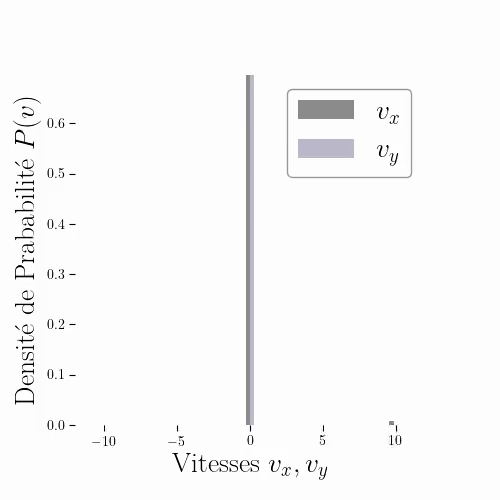
\includegraphics[width=0.33\linewidth]{figures/00_PreRemInt/frames_2D_velocity_distribution/frame_00001}
            };

            \node[above=-0.2cm of b, shift={(-2 , 0)}] {\fontsize{12pt}{14pt}\selectfont \bfseries b)};

            \node[draw = none  , rectangle , right = 0.1cm of b  ] (c)   {
                \animategraphics[
                    autoplay,
                    %loop,
                    width=0.33\linewidth, buttonsize=1em,
                ]{60}{figures/00_PreRemInt/frames_2D_velocity_distribution/frame_}{00001}{00600}
            };%
            %   \node[draw = none  , rectangle , right = 0.1cm of b  ] (c)  { %at (6,1.5)
            %     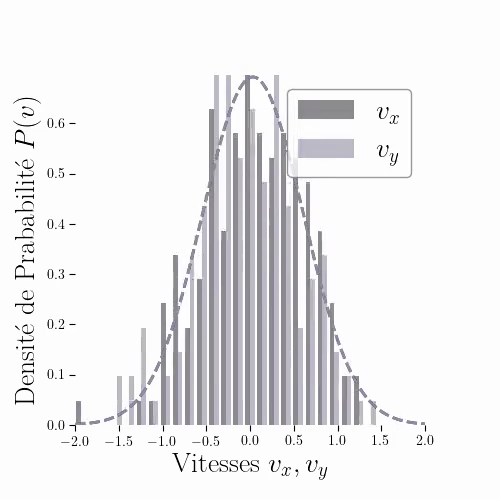
\includegraphics[width=0.33\linewidth]{figures/00_PreRemInt/frames_2D_velocity_distribution/frame_00600}
            %   };

            \node[above=-0.2cm of c, shift={(-2 , 0)}]  {\fontsize{12pt}{14pt}\selectfont \bfseries c)};

            \newcommand{\curve}{($(b)!0.1!(c) + (0,3.2)$) to[out=50,in=130] ($(b)!0.9!(c) + (0,3.2)$)}

            %Type 1
            %\def\TypeIPath{(b)to[out=50,in=140](c)}
            %\draw[opacity = 0.1 , draw=colorFive,line width=1.2ex,arrows={ -Computer Modern Rightarrow[ sharp, length=0.4cm ]}]\curve;
            \path[spath/save=TypeIPath]\curve;
            \path[spath/save global = line1] ($(b)!0.5!(c)$) --++ (-2.6,5);
            \path[spath/save global = line2] ($(b)!0.5!(c)$) --++ (2.6,5);
            \tikzset{spath/.cd,
                split at intersections with={TypeIPath}{line1},
                split at intersections with={TypeIPath}{line2},
                get components of={TypeIPath}\cpts
            }
            \draw[draw=colorFive,line width=1.2ex, spath/restore=\getComponentOf\cpts{1}] node {};
            \draw[draw=colorFive,line width=1.2ex,arrows={ -Computer Modern Rightarrow[ sharp, length=0.4cm ]},  spath/restore=\getComponentOf\cpts{3}] node {};

            \path[
            %cm={1,0,0,1,(0,-1.2cm)},
            draw=none, postaction={ decorate, decoration={ raise=0pt, text along path, text
                            align=center, text={ |\fontsize{15pt}{10pt}\selectfont\bfseries| Thermalisation
                                    ||}, text color=colorFive} }, spath/restore=\getComponentOf\cpts{2} , transform
            canvas={shift={(0,-0.2cm)}}] ;

            % \tikzset{fleche/.style={->,>=stealth',shorten >=2pt, Prune!50!colorFour,  very thick,double,double distance=20pt}}

            %\draw[fleche] \curve ;

            % \draw[->,>=Computer Modern Rightarrow,trim left=1pt,trim right=1pt,line width=0.1ex,Prune!50!colorFour] \curve ;

            % \draw[decorate,decoration={text along path,reverse path,text align=center, text color=Prune!50!colorFour, text={ {|\sffamily\fontsize{10pt}{12pt}\selectfont\bfseries| Thermalisation || . } },pre length=1cm},draw=none]\curve ;

        \end{scope}

        %\drawgrid{-0.5}{20}{-1}{20}

    \end{tikzpicture}
    \caption{a) Position des sphères dures en deux dimensions au cours du temps après avoir donné une impulsion initiale à une des sphères (sphère rouge). b) Distribution des vitesses des sphères immédiatement après l'impulsion initiale. c) Distribution des vitesses des sphères après \emph{thermalisation}, qui suit la distribution de \emph{Maxwell-Boltzmann}.\\
        Avec le logiciel Adobe acrobat Reader DC, il est possible de lancer les animations en cliquant dessus. Ces simulations sont générés grace è une code écrit en Python.
        Les codes pythons et animation sont disponible sur un des dépots github associé à ce mémoire : \url{https://github.com/THEMEZE/N-Corps-elastiques-1D-2D}. Idem pour la figure \ref{fig:hard_spheres_1D_animation}.
    }
    \label{fig:hard_spheres_2D_animation}
\end{figure}

\vspace{-0.5cm}
\subsubsection{Les sphères dures en une dimension}

Considérons maintenant le même système de sphères dures, mais contraint à une
géométrie unidimensionnelle avec conditions aux limites périodiques. Comme
précédemment, une impulsion initiale est appliquée à une particule
(figure~\ref{fig:hard_spheres_1D_animation}a). Cependant, la contrainte
cinématique imposée par l’unidimensionnalité modifie radicalement la dynamique
du système.

\smallskip

%\smallskip

%\begin{figure}[h]
\begin{wrapfigure}[22]{L}{0.50\linewidth}
    \centering
    \begin{tikzpicture}
        %\begin{scope}[transform canvas={scale=0.6}]

        \node (fig) at (0,0) {
            \begin{tikzpicture}

                \begin{scope}[shift={(0,0)}]

                    \node (a) at (0,0) {
                        \animategraphics[
                            %controls, 
                            autoplay, % démarre automatiquement 
                            %loop, % boucle infinie,
                            %palindrome, % (optionnel) rejoue à l'envers,
                            %clicktoshow, % permet de lancer/pause par clic
                            width=0.95\linewidth,
                            %buttonsize=1em,
                            poster=first
                        ]{60}{figures/00_PreRemInt/frames_1D_positions_animation/frame_}{00001}{00600}
                    }; \node[above=-0.2cm of a , shift={(-4 , 0)}] (nomA)
                    {\fontsize{12pt}{14pt}\selectfont \bfseries a)};

                    \draw [color = white] (-3,-1) rectangle +(10,2);

                    \node[draw = none , rectangle , shift={(-2 , 0)},  below = 0.5cm of a] (b)  {
                        %\multiframe{5}{i=1+1}{
                        \animategraphics[
                            autoplay,
                            loop,
                            width=0.45\linewidth, buttonsize=1em, poster=1
                        ]{60}{figures/00_PreRemInt/frames_Newton/frame_}{00001}{00043} }; %}

                    \node[below = 1.0cm of nomA , shift={(0 , 0)}] (nomB) {\fontsize{12pt}{14pt}\selectfont \bfseries b)};

                    \node[draw = none  , rectangle , right = 0.1cm of b , shift={(0 , 0)} ] (c)  { %at (6,1.5)
                        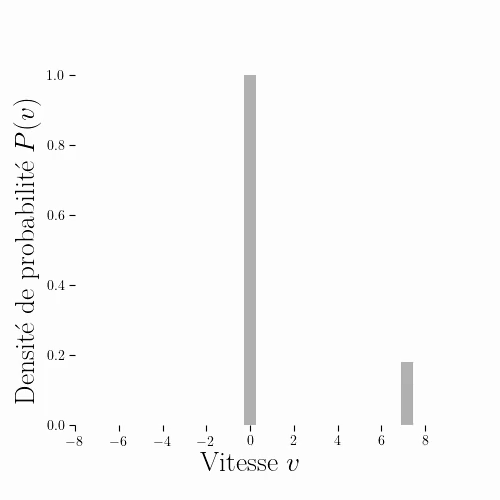
\includegraphics[width=0.45\linewidth]{figures/00_PreRemInt/frames_1D_velocity_distribution/frame_00600}
                    };

                    \node[right=4.5cm of nomB, shift={(0 , 0)}] (nomC) {\fontsize{12pt}{14pt}\selectfont \bfseries c)};

                \end{scope}
            \end{tikzpicture}
        }

        \node[below=-0.5cm of fig , shift={(-1 , 0)}] {
            \begin{minipage}{0.9\linewidth}
                \caption{a) Position des sphères dures en une dimension au cours du temps après avoir donné une impulsion initiale à une des sphères (sphère rouge). b) Illustration du \em{pendule de Newton} extrait de l'animation disponible à l'adresse : \url{https://commons.wikimedia.org/wiki/File:Newtons_cradle_animation_new.gif?uselang=fr}. c) Distribution des vitesses des sphères qui reste inchangée au cours du temps, empêchant la thermalisation.\\
                    %Avec le logiciel Adobe acrobat Reader DC, il est possible de lancer les animations en cliquant dessus.
                    %Ces simulations sont générés grace è une code écrit en Python.
                    %Les codes pythons et animation sont disponible sur un des dépots github associé à ce mémoire : \url{https://github.com/THEMEZE/N-Corps-elastiques-1D-2D}
                }
                \label{fig:hard_spheres_1D_animation}
            \end{minipage}
        };

        %\drawgrid{-5.5}{10}{-1}{3}

    \end{tikzpicture}

\end{wrapfigure}
%\end{figure}
Pour des particules identiques, une collision élastique en une dimension se
résume à un simple échange de vitesses : \( (v_i,v_j)\longrightarrow(v_j,v_i).
\) Ainsi, à tout instant, l’ensemble des vitesses est strictement conservé. La
dynamique consiste uniquement en une permutation des vitesses entre particules,
phénomène analogue à celui observé dans le \emph{pendule de Newton}
(figure~\ref{fig:hard_spheres_1D_animation}b). En particulier, la distribution
des vitesses demeure inchangée au cours du temps
(figure~\ref{fig:hard_spheres_1D_animation}c).

\smallskip

Contrairement au cas bidimensionnel, le système ne thermalise donc jamais :
aucune relaxation vers une distribution de Maxwell--Boltzmann n’a lieu. Les
quantités macroscopiques usuelles — densité de particules, densité d’impulsion,
densité d’énergie — ne suffisent plus à caractériser l’état stationnaire.
Celui-ci conserve une dépendance explicite à l’ensemble des conditions
initiales microscopiques. Plus précisément, le système possède un nombre
extensif de constantes du mouvement, égal au nombre de degrés de liberté. {\bf
La dynamique conserve donc l’intégralité de la distribution initiale des
vitesses $\boldsymbol{\tilde{n}(v)}$} .

\smallskip

On dit alors que le système est \emph{intégrable} ou \emph{non-ergodique} : la
dynamique n’explore pas ergodiquement l’espace des phases et le système
conserve une mémoire complète de son état initial: les particules ne peuvent
pas se contourner, ce qui réduit drastiquement l’espace des processus
collisionnels accessibles.%Cette absence dethermalisation résulte directement de la contrainte unidimensionnelle : 

\smallskip

Ce comportement est générique des systèmes unidimensionnels à interactions
locales, classiques comme quantiques. Beaucoup de modèles en une dimension
possèdent un ensemble extensif de charges conservées qui contraint fortement
leur dynamique hors équilibre et empêche la relaxation thermique
conventionnelle.

\smallskip

%Dans la limite thermodynamique, la dynamique peut être décrite par une équation cinétique intégrable de type Boltzmann--Enskog. Contrairement aux équations cinétiques usuelles, son intégrabilité implique l’absence d’irréversibilité effective : la distribution des vitesses reste conservée au cours du temps, traduisant l’absence de thermalisation du système.

\vspace{-0.5cm}

\subsection{Dynamique hors équilibre et intégrabilité quantique en une dimension}

%L’exemple classique des sphères dures met en évidence un point fondamental : la dynamique hors équilibre dépend de manière cruciale de la dimensionnalité et de l’intégrabilité du système. Alors que les systèmes ergodiques de dimension supérieure relaxent vers un équilibre thermique universel décrit par la mécanique statistique usuelle, les systèmes unidimensionnels intégrables conservent un nombre extensif de constantes du mouvement, ce qui contraint fortement leur dynamique et empêche la thermalisation conventionnelle.

%\smallskip

Cette absence de thermalisation ne signifie toutefois pas que la dynamique soit
triviale. Au contraire, les systèmes intégrables en une dimension présentent
une riche phénoménologie hors équilibre : une perturbation locale engendre des
modes balistiques cohérents dont la propagation est gouvernée par les lois de
conservation du système. À grande échelle spatio-temporelle, cette dynamique
peut conduire à l’émergence d’états stationnaires non thermiques décrits non
pas par l’ensemble de Gibbs canonique, mais par des {\bf \emph{Ensembles de
            Gibbs Généralisés} (\emph{Generalized Gibbs Ensembles}, \textsf{GGE})},
construits à partir de l’ensemble complet des charges conservées.

\smallskip

Dans les systèmes quantiques intégrables, ces charges conservées sont
naturellement associées aux \emph{rapidités}, variables qui caracteirse les
quasi-particules du système. %La distribution des rapidités joue alors un rôle central : elle remplace les variables thermodynamiques usuelles et caractérise complètementles états stationnaires hors équilibre.

\smallskip

La description de la dynamique à grande échelle nécessite ainsi un nouveau
cadre (développé en 2019) hydrodynamique, appelé {\bf\emph{hydrodynamique
    généralisée} (\emph{Generalized Hydrodynamics}, \textsf{GHD})}, développé
récemment pour décrire le transport et l’évolution hors équilibre des systèmes
intégrables. Dans ce formalisme, les champs hydrodynamiques usuels sont
remplacés par une infinité de densités conservées associées aux rapidités.

%\smallskip

%Le travail présenté dans cette thèse s’inscrit dans ce contexte. Avant d’aborder les résultats originaux, nous introduirons les principaux outils théoriques nécessaires à leur compréhension : le formalisme des rapidités, les Ensembles de Gibbs Généralisés décrivant les états stationnaires intégrables, ainsi que l’hydrodynamique généralisée, qui permet de décrire leur dynamique hors équilibre.

\smallskip

Mon système d’étude est constitué de $N$ bosons confinés en une dimension. Le
cas de particules bosoniques libres est aujourd’hui bien compris et peut être
décrit analytiquement. En revanche, la description devient beaucoup plus riche
lorsque le nombre de particules peut varier ou lorsque des interactions entre
bosons sont introduites.

Ces systèmes constituent un cadre particulièrement intéressant pour introduire
et motiver des outils fondamentaux de la physique moderne, comme la seconde
quantification et la théorie quantique des champs. Ils offrent également une
ouverture naturelle vers la physique statistique, discipline essentielle pour
décrire les systèmes comportant un grand nombre de degrés de liberté et les
phénomènes collectifs associés.

%L’étude des gaz quantiques unidimensionnels permet ainsi de relier des conceptsissus de plusieurs domaines de la physique théorique tout en conservant unsystème suffisamment simple pour rester analytiquement et numériquementaccessible.

\vspace{-0.5cm}
\subsubsection{État stationnaire et constante du mouvement}

\paragraph{État stationnaire.}

\EncadreDeux
{Formalisme}{{\bf \textsf{Lieb-Liniger} \textsf{(LL)}}}{woodChene}
{\paragraph*{}
    L'état stationnaire d'un système unidimensionnel de  $N$ bosons de masse $m$ en interaction ponctuelle est décrit par le {\bf modèle de \textsf{Lieb-Liniger} \textsf{(LL)}} :
    \begin{eqnarray}\label{eq.LL}
        \ptFleche{LL}{$\operator{H}$}  & = &{\color{colorFour} \underbrace{\frac{\hbar^2}{2m} \sum_{i = 1 }^{\ptFleche{Nombre}{$N$}} \operator{\partial}_{x_i}^2 }_{\text{Cinétique}}} + {\color{colorSix} \underbrace{\ptFleche{motg}{$g$} \sum_{1 \leq i < j \leq N } \operator{\delta}(x_i - x_j )  }_{\text{Interraction}}} ,
    \end{eqnarray}

    \begin{tikzpicture}[overlay]
        \draw[  opacity = 1 ]
        (LL) edge[line width=0.4ex ,color = colorOne ,arrows = {Computer Modern Rightarrow[sharp ,length=0.2cm]-},  , out = 180 , in = 0  ]node[pos=1, left]{\color{colorOne} \fontsize{8pt}{102pt}\selectfont \bfseries  Hamiltonien }($(LL) + (-2.5cm,0.0cm)$)
        ;
        \draw[  opacity = 1 ]
        (Nombre) edge[line width=0.2ex ,color = colorFour ,arrows = {Computer Modern Rightarrow[sharp ,length=0.1cm]-},  , out = 10 , in = 180  ]node[pos=1, right]{\color{colorFour} \fontsize{5pt}{102pt}\selectfont \bfseries  numbre d'atomes }($(Nombre) + (1cm,0.15cm)$)
        ;

        % \draw[  opacity = 1 ]
        %   (Cinetic) edge[line width=0.4ex ,color = colorFour ,arrows = {Computer Modern Rightarrow[sharp ,length=0.2cm]-},  , out = 150, in = 0  ]node[pos=1, left]{\color{colorFour} \fontsize{8pt}{102pt}\selectfont \bfseries  Kinetic energy }($(Cinetic) + (-1cm,1.0cm)$)
        % ;

        \draw[  opacity = 1 ]
        %(Potentiel) edge[line width=0.4ex ,color = colorSix ,arrows = {Computer Modern Rightarrow[sharp ,length=0.2cm]-},  , out = 90 , in = 180  ]node[pos=1, right]{\color{colorSix} \fontsize{8pt}{102pt}\selectfont \bfseries  Contact potential }($(Potentiel) + (1cm,1.5cm)$)
        (motg) edge[line width=0.2ex ,color = colorSix ,arrows = {Computer Modern Rightarrow[sharp ,length=0.1cm]-},  , out = -120 , in = 0  ]node[pos=1, left]{\color{colorSix} \fontsize{5pt}{102pt}\selectfont \bfseries  force de répulsion 1D }($(motg) + (-0.75cm,-1.25cm)$)
        ;

    \end{tikzpicture}

    où la première partit correspond à l’énergie cinétique des bosons, tandis que
    la seconde partie représente une interaction de contact caractérisée par une
    force de répulsion 1D $g$.}

\EncadreDeux
{Formalisme}{{\bf \textsf{Rapidité} $\boldsymbol{\theta}$}}{woodChene}{ \paragraph*{} Les {\bf
            \textsf{états stationnaires}} s'écrit

    \begin{eqnarray}\label{eq.StationaryState}
        \ptFleche{FOnde}{$\displaystyle \psi_{\ptFleche{Listetheta}{\color{colorSix} $\{\theta_a \}$}}(x_1 < \cdots <  x_N)$}
        & \propto &
        \sum_{\mathrm{perm.}\sigma}
        A_{\sigma , \color{colorSix} \{\theta_a \} } e^{i \frac{m}{\hslash}\left ( {\color{colorSix}\ptFleche{Rapiditie}{$\theta$}_{\sigma(1)}} x_1 + \cdots + {\color{colorSix}\theta_{\sigma(N)}}x_N \right )},
    \end{eqnarray}

    \begin{tikzpicture}[overlay]

        \draw[  opacity = 1 ]
        ($(FOnde) + (-2.0cm,0.0cm)$) edge[line width=0.4ex ,color = colorOne ,arrows = {Computer Modern Rightarrow[sharp ,length=0.2cm]-},  , out = 180 , in = 0  ]node[pos=1, left]{\color{colorOne} \fontsize{8pt}{102pt}\selectfont \bfseries  État }($(FOnde) + (-3.2cm,0.0cm)$)
        ;

        \draw[  opacity = 1 ]
        (Rapiditie) edge[line width=0.4ex ,color = colorSix ,arrows = {Computer Modern Rightarrow[sharp ,length=0.2cm]-},  , out = 90 , in = 180  ]node[pos=1, right]{\color{colorSix} \fontsize{8pt}{10}\selectfont \bfseries rapidité}($(Rapiditie) + (1.5cm,0.75cm)$)
        ;

        \draw[
            opacity = 1 ,
        ]
        (Listetheta) edge[
                line width=0.4ex ,
                color = colorSix ,
                arrows = {Computer Modern Rightarrow[sharp ,length=0.2cm]-},
                out = 90 , in = 180 ,
                % decorate,
                % decoration={
                %   text along path,
                %   text align=center,
                %   text={\color{\colorSix}\fontsize{6pt}{8pt}\selectfont Wavefunction}
                % },
            ]
        node[pos=1, right]
            {\color{colorSix}\fontsize{6pt}{8pt}\selectfont$\{\theta_1,\dots,\theta_N\}$}
        ($(Listetheta)+(0.5cm,0.75cm)$)
        ;
        % \draw[  opacity = 1 ]
        %       (Listetheta) edge[line width=0.4ex ,color = colorSix ,arrows = -{Computer Modern Rightarrow[sharp ,length=0.2cm]},  , out = -90 , in = 180  ]node[pos=1, right]{\color{red} \fontsize{5}{10}\selectfont \bfseries  $ \displaystyle  \ket{\{\theta_a \}}$ }($(Listetheta) + (1cm,-0.75cm)$)
        % ;

    \end{tikzpicture}

    Soit avec une somme sur des permutation d'indince (notée
    \guillemotleft{}$\sigma$\guillemotright{}). On voit apparètre des
    \guillemotleft{}$\theta$\guillemotright{} , que l'on appelle \emph{rapidités},
    homogènes à des vitesses, et qui caractérisent complètement les états
    stationnaires du système. Les rapidité sont les vittesse des quasi-particules.
    Les coefficients $A_{\sigma , \{\theta_a \} }$ sont fixés par les conditions de
    continuité de la fonction d'onde et de ses dérivées au point de contact entre
    les bosons.

}

\EncadreDeux
{Formalisme}{{\bf \textsf{Bethe Ansatz} \textsf{(BA)}}}{woodChene}{ \paragraph*{} La condition de
    periodicité des bords implique l'équation de {\bf \textsf{Bethe Ansatz} \textsf{(BA)}} :

    \begin{eqnarray}\label{eq.BA}
        \ptFleche{BA}{$\displaystyle \frac{m}{\hslash} {\color{colorSix}\theta_a} L$} + \sum_{b = 1}^N \Phi ( \theta_a - \theta_b)  & = &  2 \pi {\color{colorSix}\ptFleche{I}{ $I_a$} } \quad a = 1 , \cdots , N ,
    \end{eqnarray}

    \begin{tikzpicture}[overlay]

        \draw[  opacity = 1 ]

        ($(BA) + (-0.5cm,0.0cm)$) edge[line width=0.4ex ,color = colorOne ,arrows = {Computer Modern Rightarrow[sharp ,length=0.2cm]-},  , out = 180 , in = 0  ]node[pos=1, left]{\color{colorOne} \fontsize{8pt}{10}\selectfont \bfseries Équation de Bethe Ansatz}($(BA) + (-1.5cm,0cm)$)%periodic boundary condition

        ($(I) + (0cm,0.2cm)$) edge[line width=0.4ex ,color = colorSix ,arrows = {Computer Modern Rightarrow[sharp ,length=0.2cm]-},  , out = 90 , in = 180  ]node[pos=1, right]{\color{colorSix} \fontsize{6pt}{10}\selectfont \bfseries entiers de Bethe $\displaystyle  I_a \in
            \left\{
            \begin{array}{rrl}
                \mathbb{Z} + \dfrac{1}{2} & \text{si}    & N \in 2\mathbb{N}       \\
                \mathbb{Z}                & \text{sinon} & (N \in 2\mathbb{N} + 1)
            \end{array}
            \right.$ }($(I) + (0.25cm,0.75cm)$)

        ;
    \end{tikzpicture}
    où $L$ est la taille du système, $\Phi(\theta) = 2 \arctan(\theta / (g/\hbar))$ est la phase de diffusion entre les quasi-particules, et $\{I_a\}$ sont des entiers ou demi-entiers appelés \emph{entiers de Bethe}, qui indexent les solutions de l’équation de \textsf{Bethe Ansatz}. La connaissance de ces rapidités permet de caractériser complètement les états stationnaires du système, et joue un rôle central dans la description de sa dynamique hors équilibre.
    %}
}

\vspace{-0.0cm}
\begin{wrapfigure}[18]{R}{0.50\linewidth}
    \centering
    \begin{tikzpicture}
        %\begin{scope}[transform canvas={scale=0.6}]

        \node[shift={(0 , 0)}] (fig) {
            \begin{tikzpicture}
                \begin{scope}[shift={(0,0)}]

                    \node (a) at (0,0) {

                        \begin{animateinline}[autoplay,width=0.95\linewidth,
                                buttonsize=1em,
                                poster=13]{2}

                            \multiframe{13}{i=1+1}{
                                \includegraphics[
                                    page=\i,
                                    width=1.0\linewidth
                                ]{figures/Figures_BA_Thermo.pdf}
                            }

                        \end{animateinline}

                    }; %\node[above=-0.2cm of a , shift={(-2 , 0)}]{\fontsize{12pt}{14pt}\selectfont \bfseries a)};

                \end{scope}
            \end{tikzpicture}

        }

        \node[below=-0.7cm of fig , shift={(0 , 0)}] {
            \begin{minipage}{0.9\linewidth}
                \caption{Illustration de l'{\bf équation \textsf{(BA)}}.}
                \label{fig:eqBA}
            \end{minipage}
        };

        %\drawgrid{-0.5}{10}{-1}{3}

    \end{tikzpicture}

\end{wrapfigure}

Construisons l’axe des entiers de {\bf \textsf{Bethe}} $\boldsymbol{I_a}$,
espacés d’une unité. À l’état fondamental, ces entiers sont consécutifs et
centrés autour de zéro. Les excitations du système correspondent alors soit à
la création de trous dans cette distribution, soit à l’ajout d’entiers en
dehors de la mer fondamentale (cf. fig.~\ref{fig:eqBA}).

\smallskip

Les {\bf équations \textsf{(BA)}} (cf. eq.~\eqref{eq.BA}) établissent une
correspondance entre les entiers de Bethe $I_a$ et les rapidités $\theta_a$.
Dans la limite thermodynamique, \( L \to \infty, \quad N \to \infty, \quad N/L
= \text{cste}, \) les rapidités deviennent distribuées continûment. Un
intervalle $[\theta,\theta+\delta\theta[$ correspond alors à un intervalle
$[I,I+\delta I[$ de l’axe des entiers de Bethe tel que \(
L\,\rho_s(\theta)\,\delta\theta = \delta I, \) où $\rho_s(\theta)$ désigne la
densité d’états en rapidité. Le nombre de quasi-particules dans cet intervalle
est quant à lui donné par \( L\,\rho(\theta)\,\delta\theta, \) où
$\rho(\theta)$ est la densité de rapidités occupées.

\smallskip

Ainsi, dans la limite thermodynamique, un état macroscopique intégrable est
entièrement caractérisé par la fonction de distribution des rapidités
$\rho(\theta)$. Il est également commode d’introduire le facteur d’occupation
\( \nu(\theta)=\frac{\rho(\theta)}{\rho_s(\theta)}, \) qui représente la
fraction d’états occupés à la rapidité $\theta$.

\paragraph{Comment mesurer la distribution des rapidités ? Et ressemble à quoi ?}

Les rapyditées ne sont pas les vitesses des particule donc la distribution de
rapidités $\rho(\theta)$ ne doit pas être confondue avec la distribution des
vitesses des bosons $\tilde n(v)$. Cependant, dans un protocole d’expansion
libre, ces deux distributions deviennent directement liées.

%\smallskip

\begin{wrapfigure}[10]{L}{0.28\linewidth}
    \centering
    \begin{tikzpicture}
        %\begin{scope}[transform canvas={scale=0.6}]

        \node[shift={(0 , 0)}] (fig) {
            { %at (6,1.5)
                    \includegraphics[page=11,width=0.95\linewidth]{figures/Figures.pdf}
                }
        };

        \node[below=-0.3cm of fig , shift={(0 , 0)}] {
            \begin{minipage}{0.9\linewidth}
                \captionof{figure}{Illustration de la trajectoires de bosons.}
                \label{fig:protocole}
            \end{minipage}
        };

        %\drawgrid{-0.5}{10}{-1}{3}
    \end{tikzpicture}

    %\label{fig:protocole}
\end{wrapfigure}
\subparagraph{Protocole.}
Considérons un gaz initialement confiné dans une boîte de taille $L$. À
l’instant $t=0$, le confinement est supprimé. Les particules interagissent
encore pendant un temps transitoire, puis l’expansion dilue le système et les
collisions deviennent négligeables. À long temps, les bosons se propagent donc
balistiquement, et leur distribution asymptotique de vitesses converge vers la
distribution de rapidités : \( \tilde
n(v)\underset{t\to\infty}{\longrightarrow}L\,\rho(v). \) (cf.
fig.~\ref{fig:protocole}).

\smallskip

Expérimentalement, cette distribution est accessible par mesure de la densité
spatiale après temps de vol (\emph{time-of-flight}). En effet, à long temps,
position et vitesse deviennent proportionnelles : \( x\simeq v\tau , \) de
sorte que
\begin{eqnarray}
    \tau\, n(x,\tau)
    \underset{\tau\to\infty}{\longrightarrow}
    \tilde n(x/\tau)
    \underset{\tau\to\infty}{\longrightarrow}
    L\,\rho(x/\tau).
\end{eqnarray}
Ainsi, la mesure de la distribution asymptotique de densité permet d’accéder
directement à la distribution de rapidités.

\smallskip

\subparagraph{La distribution de rapidités ressemble a quoi ?}
À l’état fondamental, le facteur d’occupation $\nu$ vaut $1$ pour $|\theta|<\theta_F$ et $0$ ailleurs (cf. fig.~??), où $\theta_F$
désigne la rapidité de Fermi. La forme de la distribution de rapidités est
contrôlée par le paramètre d’interaction de Lieb--Liniger
\(
\gamma=\frac{mg}{\hbar^2 n}.
\)

\smallskip

Dans la limite de sphère dure ou de Tonks--Girardeau ($\gamma\to\infty$), les
bosons fortement répulsifs se fermionisent : la distribution de rapidités
coïncide alors avec celle d’un gaz de fermions libres à température nulle,
présentant une structure de type Fermi--Dirac à bord franc (cf.
fig.~\ref{fig:eqBA}). À mesure que $\gamma$ diminue, les équations du Bethe
Ansatz prédisent une déformation continue de cette distribution. Dans le régime
de condensat ou de Gross--Pitaevskii ($\gamma\to0$), la distribution de
rapidités tend vers une forme en demi-cercle (cf. fig.~\ref{fig:eqBA}). Hors
équilibre ou à température finie, le facteur d’occupation $\nu(\theta)$ peut
prendre continûment des valeurs entre $0$ et $1$, sans bord de Fermi net.

\smallskip

La distribution de rapidités $\rho(\theta)$ — ou, de manière équivalente, le
facteur d’occupation $\nu(\theta)$ — caractérise complètement l’état
macroscopique après relaxation. Les observables hydrodynamiques usuelles
s’obtiennent comme moments de cette distribution : \( \int \mathrm d\theta\,
\rho(\theta)=n, \) \( \int \mathrm d\theta\, m\theta\,\rho(\theta)=p, \) \(
\int \mathrm d\theta\, m\theta^2\,\rho(\theta)=e, \) respectivement les
densités de particules, d’impulsion et d’énergie. Les moments d’ordre supérieur
génèrent les autres charges conservées du système intégrable. L’état
stationnaire est ainsi décrit non par un {\bf \emph{Ensemble de Gibbs}
        \textsf{(GE)}} thermique usuel, mais par un {\bf \emph{Ensemble de Gibbs
            Généralisé} \textsf{(GGE)}}, construit à partir de l’ensemble complet des
charges conservées.

\vspace{-0.5cm}
\subsubsection{Dynamique}
%\begin{figure}[h]
\begin{wrapfigure}[12]{r}{0.3\linewidth}
    \centering

    \begin{tikzpicture}

        \node (fig) {
            \includegraphics[
                page=5,
                width=0.95\linewidth
            ]{figures/Figures.pdf}
        };

        \node[
            below=-0.2cm of fig
        ] {

            \begin{minipage}{0.9\linewidth}
                \captionof{figure}{
                    Illustration des échelles macroscopique,
                    mésoscopique et microscopique.
                }
                \label{fig:echeuler}
            \end{minipage}

        };
        %\drawgrid{-0.5}{10}{-1}{3}

    \end{tikzpicture}

\end{wrapfigure}
% \begin{wrapfigure}[15]{r}{0.28\linewidth}

%     \centering

%     \includegraphics[
%         page=5,
%         width=\linewidth
%     ]{figures/Figures.pdf}

%     \caption{
%         Illustration des échelles macroscopique,
%         mésoscopique et microscopique.
%     }

%     \label{fig:echeuler}

% \end{wrapfigure}
%\end{figure}

Nous souhaitons maintenant passer de la description thermodynamique à une
description hydrodynamique, c’est-à-dire étudier des systèmes macroscopiques
inhomogènes à grande échelle spatiale et temporelle. Pour cela, on introduit
une décomposition en cellules fluides mésoscopiques : chaque cellule est
suffisamment grande pour contenir un nombre macroscopique de particules, mais
suffisamment petite pour que les grandeurs locales y soient quasi uniformes.
Cette approche repose sur une séparation d’échelles entre la dynamique
microscopique et les variations macroscopiques du système
(fig.~\ref{fig:echeuler}) .

\smallskip

À l’échelle d’Euler, on néglige les variations spatiales microscopiques ainsi
que les effets diffusifs, et l’on ne conserve que les contributions dominantes
à grande distance et à grand temps. Dans un système ergodique (chaotique),
l’état local d’une cellule fluide est entièrement décrit par les champs
hydrodynamiques conservés :
\(
n(\mathbf{x};t),\,
p(\mathbf{x};t),\,
e(\mathbf{x};t),
\)
correspondant respectivement aux densités locales de particules, d’impulsion et
d’énergie.

\smallskip

Dans un système intégrable, cette description est insuffisante : chaque cellule
fluide est caractérisée par une distribution locale de rapidités \(
\rho(x,\theta;t), \) c’est-à-dire par une infinité de densités conservées
paramétrées par la rapidité $\theta$.

\smallskip

L’évolution temporelle de ces quantités est déterminée par leur transport entre
cellules fluides et s’écrit sous la forme d’équations locales de conservation,
ou équations de continuité. À l’échelle d’Euler, ces relations constituent les
équations hydrodynamiques du système, analogues aux équations d’Euler de la
mécanique des fluides.

\smallskip

%\paragraph{formalisme de l'\emph{Ensemble de Gibbs Généralisé} (GGE).}
Avant d'aborder la dynamique, on introduit le formalisme du {\bf
        \textsf{(GGE)}} :

\EncadreDeux
{Formalisme}{{\bf \textsf{Ensemble de Gibbs Généralisé} \textsf{(GGE)}}}{woodChene}{\paragraph*{Opérateurs charges
        globales}
    On définit les opérateurs \emph{charges globales} comme des fonctionnelles
    linéaires agissant sur une fonction réelle et régulière $f(x,\theta)$ définie
    sur $\mathbb{R}^2$, selon
    \begin{equation}\label{chap:GHD:eq.charge.global.0}
        \ptFleche{OCGL}{$\displaystyle\operator{\mathcal{Q}}[f]$}
        = \int_{\mathbb{R}^2} dx\, d\theta\, f(x, \theta)\, \! \! \! \ptFleche{ODR}{$\displaystyle \color{colorSix} \operator{\rho}(x, \theta ; t)$},
    \end{equation}

    \begin{tikzpicture}[overlay]

        \draw[  opacity = 1 ]
        ($(OCGL) + (-0.50cm,0.0cm)$) edge[line width=0.4ex ,color = colorOne ,arrows = {Computer Modern Rightarrow[sharp ,length=0.2cm]-},  , out = 180 , in = 0  ]node[pos=1, left]{\color{colorOne} \fontsize{8pt}{102pt}\selectfont \bfseries  Opérateur charge globale linèaire }($(OCGL) + (-1.2cm,0.0cm)$)
        ;

        \draw[  opacity = 1 ]
        (ODR) edge[line width=0.2ex ,color = colorSix ,arrows = {Computer Modern Rightarrow[sharp ,length=0.1cm]-},  , out = 90 , in = 180  ]node[pos=1, right , draw = none  , rectangle ]{\color{colorSix} \fontsize{4pt}{4}\selectfont \bfseries $\displaystyle \operator{\rho}(x, \theta ; t) \ket{\{\theta_a\}} = \! \! \!  \ptFleche{DR}{$\displaystyle\rho(x, \theta ; t)$}  \! \! \! \ket{\{\theta_a\}}$ }($(ODR) + (0.5cm,0.75cm)$)
        ;

        \draw[  opacity = 1 ]
        (DR) edge[line width=0.2ex ,color = colorSix ,arrows = {Computer Modern Rightarrow[sharp ,length=0.1cm]-},  , out = -90 , in = 90  ]node[pos=1, below , draw = none  , rectangle , shift = {(0cm , 0.25cm)}]{\color{colorSix} \fontsize{4pt}{4}\selectfont \bfseries $\displaystyle \sum_{a = 1}^N \delta ( x - x_a) \delta ( \theta  - \theta_a)$ }($(DR) + (-0cm,-0.5cm)$)
        ;

    \end{tikzpicture}
    où $\operator{\rho}(x,\theta ; t )$ est l'opérateur distribution de rapidité, diagonale dans la base des configurations $\ket{\{\theta_a\}}$.
    Cette quantité correspond à la charge totale associée à une observable prenant
    la valeur $f(x,\theta)$ pour chaque quasi-particule.\footnote{ \EncadreDeux
        {Information}{{\bf \textsf{} \textsf{}}}{woodChene}{
            \noindent\textbf{Remarque~:} pour que $\operator{\mathcal{Q}}[f]$ soit
            strictement conservée dans le temps, la fonction $f$ doit être indépendante de
            $x$, c’est-à-dire $f(x,\theta) = f(\theta)$. Si $f$ dépend de $x$,
            $\operator{\mathcal{Q}}[f]$ n’est pas nécessairement conservée au cours de
            l’évolution du système. En revanche, si $f$ dépend uniquement de $\theta$ ,
            alors $\operator{\mathcal{Q}}[f]$ correspond à une véritable charge conservée.
            Dans le cadre de ce chapitre, la dépendance en $x$ est introduite pour
            faciliter certaines dérivations et l’étude des profils locaux, mais la
            conservation stricte n’est garantie que pour les fonctions $f(\theta)$
            indépendantes de $x$. } }

    \medskip

    %La valeur moyenne $\langle \operator{\mathcal{Q}}[f]\rangle_{\operator{\varrho}[w]} = \mathrm{Tr} \left[ \operator{\varrho}[w]\cdot \operator{\mathcal{Q}}[f] \right]$. 
    La {\color{colorOne} \fontsize{8pt}{8pt}\selectfont \bfseries \emph{matrice
                densité globale} $\operator{\varrho}[w]$} et la {\color{colorOne}
            \fontsize{8pt}{8pt}\selectfont \bfseries \emph{fonction de partition} $Z[w]$}
    et la {\color{colorOne} \fontsize{8pt}{8pt}\selectfont \bfseries \emph{valeur
                moyenne} $\langle \operator{\mathcal{Q}}[f]\rangle_{\operator{\varrho}[w]}$}
    s’écrivent
    \begin{equation}\label{chap:GHD:eq.charge.global.2}
        \operator{\varrho}[w] = \frac{1}{Z[w]}\, e^{-\operator{\mathcal{Q}}[w]},\qquad
        Z[w] = \mathrm{Tr} \left[ e^{-\operator{\mathcal{Q}}[w]} \right],\qquad
        \langle \operator{\mathcal{Q}}[f]\rangle_{\operator{\varrho}[w]} = \mathrm{Tr} \left[ \operator{\varrho}[w]\cdot \operator{\mathcal{Q}}[f] \right],
    \end{equation}
    où la charge globale $\operator{\mathcal{Q}}[w]$ est définie par~\eqref{chap:GHD:eq.charge.global.0}, et $w$ désigne le poids spectral.
}

Par exemple, si le système est thermostaté à une température $T$, et que sa
taille $L$ ainsi que le nombre de particules $N$ sont fixés, alors le poids
spectral s’écrit \( w(\theta) = \beta \, \varepsilon(\theta), \) où
$\varepsilon(\theta) = \tfrac{1}{2} m \theta^2$ est l’énergie par
quasi-particule, et $\beta = (k_B T)^{-1}$. Injecté dans
l’équation~\eqref{chap:GHD:eq.charge.global.2}, ce choix définit un
\emph{ensemble canonique}. Si maintenant le système est en contact avec un
réservoir de particules, le nombre de particules n’est plus fixé, mais le
potentiel chimique $\mu$ l’est. Le poids spectral devient alors \( w(\theta) =
\beta \bigl(\varepsilon(\theta) - \mu\bigr), \) et, injecté dans
l’équation~\eqref{chap:GHD:eq.charge.global.2}, il définit un \emph{ensemble
    grand canonique}. Dans ces deux cas, on parle d’\emph{ensemble de Gibbs}. Pour
rester cohérent avec les notations introduites précédemment, on peut réécrire
ces expressions sous la forme \( w(\theta) = \beta_0 f_0(\theta) + \beta_2
f_2(\theta), \) avec \( f_0(\theta) = 1, \, f_2(\theta) = \tfrac{1}{2} m
\theta^2, \, \beta_0 = -\beta \mu, \, \beta_2 = \beta. \) Cette écriture
suggère naturellement la généralisation \( w(\theta) = \sum_i \beta_i
f_i(\theta), \) qui constitue le point de départ de l’\emph{ensemble de Gibbs
    généralisé}. Les coefficients $\beta_i$ apparaissent comme des multiplicateurs
de Lagrange lors de la maximisation de l’entropie sous contraintes. Ils
imposent les valeurs moyennes des charges, \( \langle
\operator{\mathcal{Q}}[f_i] \rangle_{\operator{\varrho}[w]} = \mathrm{Tr}
\left[ \operator{\varrho}[w] \cdot \operator{\mathcal{Q}}[f_i] \right]. \)

%\medskip

\newpage

Nous allons maintenant considérer la limite thermodynamique, où les moyennes
des opérateurs sont notées sans chapeau.

%\vspace{-1cm}

\EncadreDeux
{Formalisme}{{\bf \textsf{} \textsf{}}}{woodChene}{
    \paragraph*{Limite thermodynamique.}
    Dans notre étude de la dynamique, nous n’avons pas besoin de l’information détaillée sur le poids spectral $w$.
    Dans la limite thermodynamique, nous noterons donc, les moyennes des opérateurs en supprimant leur chapeau, \emph{i.e.}
    \(
    \underset{\mathrm{therm}}{\lim} \, \langle \operator{\mathcal{O}} \rangle_{\varrho[w]} \; \equiv \; \mathcal{O},
    \)
    de sorte que, dans cette limite, la moyenne de la charge globale s’écrit
    \begin{equation}\label{chap:GHD:eq.charge.global.1}
        \ptFleche{MTOCGL}{$\displaystyle\mathcal{Q}[f]$}
        = \int_{\mathbb{R}^2} dx\, d\theta\, f(x, \theta)\, \! \! \! \ptFleche{MTDR}{$\displaystyle \color{colorSix}\rho(x, \theta ; t )$},
    \end{equation}
    \begin{tikzpicture}[overlay]

        \draw[  opacity = 1 ]
        ($(MTOCGL) + (-0.50cm,0.0cm)$) edge[line width=0.4ex ,color = colorOne ,arrows = {Computer Modern Rightarrow[sharp ,length=0.2cm]-},  , out = 180 , in = 0  ]node[pos=1, left]{\color{colorOne} \fontsize{8pt}{102pt}\selectfont \bfseries  $\displaystyle \boldsymbol{\underset{\mathrm{therm}}{\lim} \, \langle \operator{\mathcal{Q}}[f] \rangle_{\varrho[w]}}$ }($(MTOCGL) + (-1.75cm,0.0cm)$)
        ;

        \draw[  opacity = 1 ]
        (MTDR) edge[line width=0.2ex ,color = colorSix ,arrows = {Computer Modern Rightarrow[sharp ,length=0.1cm]-},  , out = 10 , in = 180  ]node[pos=1, draw = none , right=0.00cm , ellipse  , shift = {(0.00cm , -0.0cm)} ]{\color{colorSix} \fontsize{4pt}{4}\selectfont \bfseries $\mathrm{\underset{\mathrm{therm}}{\lim} \, \langle \operator{\mathcal{\rho}}(x,\theta ; t) \rangle_{\varrho[w]}}$ }($(MTDR) + (2.0cm,0.0cm)$)
        ;

    \end{tikzpicture}
    où $f$ est une fonction régulière sur $\mathbb{R}^2$.
}
%Avec ce formalisme, en appliquant $(x',\theta) \mapsto \delta(x' -x)f_i(\theta)$ dans \eqref{chap:GHD:eq.charge.global.1}, nous pouvons définirla moyenne des densités locales $q_i(x,t) = \mathcal{Q} \big[ (x',\theta) \mapsto \delta(x' - x) \, f_i(\theta) \big]$ comme
\setlength{\intextsep}{-3pt}%
\setlength{\columnsep}{-0pt}%
\begin{wrapfigure}[17]{r}{0.25\linewidth}
    \centering

    \begin{tikzpicture}

        \node (fig) {

            \begin{tikzpicture}
                \node (a) {
                    \includegraphics[
                        page=7,
                        width=1.0\linewidth
                    ]{figures/Figures.pdf}
                }
                \node[above=0.4cm of a, shift={(-2.5 , -0.4)}] (noma) {\fontsize{12pt}{14pt}\selectfont \bfseries a)};
                \node[below=0.5cm of a, shift={(0 , 0)}] (d) {
                    \includegraphics[
                        page=10,
                        width=1\linewidth
                    ]{figures/Figures.pdf}
                }
                \node[above=0.1cm of d, shift={(-2 , -0.6)}] (nomd) {\fontsize{12pt}{14pt}\selectfont \bfseries b)};

            \end{tikzpicture}
        };

        \node[
            below=-0.2cm of fig,
            shift={(-0.0 , -0)}
        ] {

            \begin{minipage}{0.9\linewidth}
                \captionof{figure}{
                    a) Diagramme $\rho(x,\theta)$.
                    b) Trasjectoires de sphères dure.
                }
                \label{fig:Pi1}
            \end{minipage}

        };
        %\drawgrid{-0.5}{10}{-1}{3}

    \end{tikzpicture}

\end{wrapfigure}
En appliquant dans \eqref{chap:GHD:eq.charge.global.1} la fonction test
\((x',\theta)\mapsto \delta(x'-x)f(\theta)\), on définit les densités locales
associées aux charges conservées :
\begin{equation}\label{chap:GHD:eq.chochet.bonnemain.4.11}
    q_{[f]}(x;t) \doteq \mathcal{Q} \big[ (x',\theta) \mapsto \delta(x' - x) \, f(\theta) \big] =  \int d\theta\, f(\theta)\,\rho(x,\theta;t).
\end{equation}
Par exemple, avec ce formalisme, les densités locales usuelles $n(x,t)$,
$p(x;t)$ et $e(x;t)$ s’écrivent comme des cas particuliers de $q_{[f_i]}(x;t)$;
respectivement avec $f_0(\theta) = 1$, \( f_1(\theta) = m \theta \) et
$f_2(\theta) = \tfrac{1}{2} m \theta^2$.
%La densité de particules $n(x,t)$, la densité d’impulsion $p(x;t)$ et la densité d’énergie $\varepsilon(x;t)$
%Les densités correspondent respectivement à avec $i \in \{0,1,2\}$
%\(q_{[f_i]}(x;t)= \mathcal{Q} \big[ (x',\theta) \mapsto \delta(x' - x) \,
%    f_i(\theta) \big] \) .

\paragraph{Formalisme de l'équation d'\emph{Hydrodynamique Généralisé} (GHD).}

Dans chaque tranche $[\theta , \theta + \delta \theta [$ , le nombre de
rapiditée $\Pi(\theta)\, \delta \theta = \mathcal{Q} \big[ (x,\theta') \mapsto
        \delta(\theta' - \theta) \, \delta \theta \big] \int dx \rho ( x , \theta ; t )
    \, \delta \theta$ ,
% \begin{eqnarray*}
%     \Pi(\theta)\, \delta \theta  =  \int dx \rho ( x , \theta ; t ) \, \delta \theta
% \end{eqnarray*}
est conservée (fig~\ref{fig:Pi1} (a)). Lorsque $\delta \theta$ tend vers $0$,
ces conservantion se transforme en \emph{Équation d'Euler} sans potentiel
extérieur : \( \partial_t \rho( x , \theta ; t ) + \partial_x j ( x, \theta ; t
) = 0 \quad \forall \theta . \) Si le système subi un potentiel extérieur
$V(x)$, certaine quasi-particule vont traverser les tranche $[\theta , \theta +
    \delta \theta [$ traduisant un flux selon $\theta$. On note $h(x,\theta) =
    \varepsilon(\theta) + V(x) $ la densité de l'hamiltonien \emph{nu} telle que
l'énergie totale moyenne s'écrit $H = \mathcal{Q}[h]$. Avec un peu de
formalisme pour les {\em crochets de Poisson} $ \{ \bullet , \bullet \}$
\footnote{ Le crochet de Poisson entre deux charges $\mathcal{Q}[f]$ et
    $\mathcal{Q}[g]$ prend la forme
    \begin{eqnarray}\label{chap:GHD:eq.chochet.bonnemain.2}
        \{\mathcal{Q}[f], \mathcal{Q}[g]\} &  \doteq   & -\int_{\mathbb{R}^2} dx\,d\theta\;\frac{\nu}{2\pi}\, \left[ \partial_x \left( \frac{\delta \mathcal{Q}[f]}{\delta \rho(x,\theta)} \right)\left( \partial_\theta \left( \frac{\delta \mathcal{Q}[g]}{\delta \rho(x,\theta)} \right) \right)^{\mathrm{dr}}_{[\nu]}-\partial_x \left( \frac{\delta \mathcal{Q}[g]}{\delta \rho(x,\theta)} \right)\left( \partial_\theta \left( \frac{\delta \mathcal{Q}[f]}{\delta \rho(x,\theta)} \right) \right)^{\mathrm{dr}}_{[\nu]}\right],\\
        & \ptFleche{E1}{$\displaystyle=$} & -\int_{\mathbb{R}^2} dx\, d\theta\, \frac{\nu}{2\pi}\left[ \partial_x f \, (\partial_\theta g)^{\mathrm{dr}}_{[\nu]}- \partial_x g \, (\partial_\theta f)^{\mathrm{dr}}_{[\nu]} \right]
        \ptFleche{E2}{$\displaystyle=$}
        \int_{\mathbb{R}^2} dx\, d\theta\, f \left[ \partial_x \left (  \, \frac{\nu}{2\pi} \, (\partial_\theta g)^{\mathrm{dr}}_{[\nu]} \right ) - \partial_\theta \left (  \, \frac{\nu}{2\pi} \, (\partial_x g)^{\mathrm{dr}}_{[\nu]} \right ) \right]
        .
    \end{eqnarray}
    \begin{tikzpicture}[overlay]

        \draw[  opacity = 1 ]
        ($(E1) + (-0.1cm,0.1cm)$) edge[line width=0.2ex ,color = colorSix ,arrows = {Computer Modern Rightarrow[sharp ,length=0.1cm]-},  , out = 150 , in = 0  ]node[pos=1, left]{\color{colorSix} \fontsize{4pt}{2pt}\selectfont \bfseries  \eqref{chap:GHD:eq.charge.global.0} }($(E1) + (-2.75cm,0.0cm)$)
        ;

        \draw[  opacity = 1 ]
        (E2) edge[line width=0.2ex ,color = colorSix ,arrows = {Computer Modern Rightarrow[sharp ,length=0.1cm]-},  , out = -90 , in = 180  ]node[pos=1, draw = none , right , rectangle  , shift = {(0.00cm , -0.0cm)} ]{\color{colorSix} \fontsize{4pt}{4pt}\selectfont \bfseries $\int dx\, d\theta \; \nu \, f \, g^{\mathrm{dr}}_{[\nu]}
            = \int dx\, d\theta \; \nu \, f^{\mathrm{dr}}_{[\nu]} \, g,$ + IPP }($(E2) + (0.2cm,-0.5cm)$)
        ;

    \end{tikzpicture}

},
l'opération \emph{habillée} $(\bullet)^{\mathrm{dr}}_{[\nu]}$
\footnote{
À toute fonction $f(\theta)$, on associe sa version \emph{habillée} (ou \emph{dressed}) $f^{\mathrm{dr}}_{[\nu]}(\theta)$, définie comme la solution de l’équation intégrale suivante :
\begin{equation}\label{eq:dressing}
    f^{\mathrm{dr}}_{[\nu]}(\theta)
    \;=\; f(\theta) \;+\; \frac{1}{2\pi}\,\bigl(\Delta \star [\nu\, f^{\mathrm{dr}}]\bigr)(\theta) = f(\theta) \;+\; \frac{1}{2\pi} \int \Delta (\theta - \theta') \nu(\theta') f^{\mathrm{dr}}_{[\nu]}(\theta') \, d\theta'  .
\end{equation}

Ici, $\nu(\theta)$ est le \textbf{facteur d’occupation}, et $\Delta/2\pi$ est
le \textbf{noyau de diffusion} caractéristique du modèle considéré avec
$\Delta(\theta) = \frac{\hbar}m \Phi'(\theta)$. Cette opération permet
d'inclure les interactions entre particules.

% On note $h(x,\theta)$ la densité de l'hamiltonien \emph{nu} telle que
% \begin{equation}\label{chap:GHD:eq.ham.1}
%     H = \mathcal{Q}[h].
% \end{equation}
% Dans notre cas $h(x,\theta) = \varepsilon(\theta) + V(x)$.
La densité d'état $\rho_s$, la distribution de rapidités , la fonction
d’occupation $\nu$, la vitesse effective $v^{\mathrm{eff}}_{[\nu]}$ et
l’accélération effective $a^{\mathrm{eff}}_{[\nu]}$ sont réliés par
\begin{equation}\label{chap:GHD:eq.nu.v.a.1}
    2 \pi \rho_s =  \frac{m}{\hbar} \, 1^{\mathrm{dr}}_{[\nu]}  ,
    \quad
    2 \pi \rho =  \frac{m}{\hbar} \, 1^{\mathrm{dr}}_{[\nu]} \, \nu ,
    \quad 2 \pi \, m \, v^{\mathrm{eff}}_{[\nu]} \, \rho  = \frac{m}{\hbar} \, (\partial_\theta h )^{\mathrm{dr}}_{[\nu]} \, \nu ,
    \quad 2 \pi \, m \, a^{\mathrm{eff}}_{[\nu]} \, \rho  = -\frac{m}{\hbar} \, (\partial_x h )^{\mathrm{dr}}_{[\nu]}\, \nu .
\end{equation}
%toutes trois étant des fonctions de $\rho(\cdot,\cdot,t)$
},
l’{\em équation de Liouville}
\footnote{
    \begin{equation}\label{chap:GHD:eq.Liouv.1}
        \frac{d q}{dt}
        = \frac{\partial q}{\partial t } + \hbar^{-1} \, \{ q , H \} = 0.
    \end{equation}
}
,

\EncadreDeux
{Formalisme}{{\bf \textsf{Équation d'Euler Généralisées} \textsf{}}}{woodChene}{
on trouve la forme de convection (\emph{Équation d'Euler} avec potentiel extérieur) :
\begin{equation}\label{chap:GHD:eq.conserv.2}
    \partial_t q_{[f]} + \partial_x j_{[f]} = F_{[f]},
\end{equation}
où le flux $j_{[f]}$ et le terme de force $F_{[f]}$ (provenant d’éventuels champs externes) sont donnés par
\begin{equation}\label{chap:GHD:eq.conserv.2.1}
    j_{[f]} = \int_{\mathbb{R}} d\theta \;  v^{\mathrm{eff}}_{[\nu]} \, f \, \rho,
    \quad F_{[f]} =  \int_{\mathbb{R}} d\theta \;  a^{\mathrm{eff}}_{[\nu]} \, f' \, \rho = - \int_{\mathbb{R}} d\theta \;   f \, \partial_\theta \left ( a^{\mathrm{eff}}_{[\nu]} \,  \rho \right ),
\end{equation}
avec $m \, v^{\mathrm{eff}}_{[\nu]} = (\partial_\theta h )^{\mathrm{dr}}_{[\nu]}/1^{\mathrm{dr}}_{[\nu]}$ et $m \, a^{\mathrm{eff}}_{[\nu]} = -(\partial_x h )^{\mathrm{dr}}_{[\nu]}/1^{\mathrm{dr}}_{[\nu]}$.
}
\EncadreDeux
{Formalisme}{{\bf \textsf{} \textsf{(GHD)}}}{woodChene}{
    De manière analogue, pour la distribution de rapidité à l’équilibre
    thermodynamique, notée \( \rho(x,\theta) = q_{[f\colon \theta' \mapsto
                    \delta(\theta'-\theta) ]} = \mathcal{Q}\big[ (x',\theta') \mapsto
        \delta(x'-x)\,\delta(\theta'-\theta) \big], \) on obtient l’\emph{équation
        d’hydrodynamique généralisée} :
    \begin{equation}\label{chap:GHD:eq.conserv.3}
        \partial_t \rho
        + \partial_x \big( v^{\mathrm{eff}}_{[\nu]}\, \rho \big)
        + \partial_\theta \big( a^{\mathrm{eff}}_{[\nu]}\, \rho \big)
        = 0.
    \end{equation}
}
\setlength{\intextsep}{-0pt}%
\setlength{\columnsep}{-0pt}%
\begin{wrapfigure}[27]{r}{0.27\linewidth}
    \centering

    \begin{tikzpicture}

        \node (fig) {

            \begin{tikzpicture}
                \node[] (b) {
                    \includegraphics[
                        page=8,
                        width=1\linewidth
                    ]{figures/Figures.pdf}
                }
                \node[above=0.1cm of b, shift={(-1 , -0.6)}] (nomb) {\fontsize{12pt}{14pt}\selectfont \bfseries a)};
                \node[below=0.5cm of b, shift={(0 , 0)}] (c) {
                    \includegraphics[
                        page=9,
                        width=1\linewidth
                    ]{figures/Figures.pdf}
                }
                \node[above=0.1cm of c, shift={(-1 , -0.6)}] (nomc) {\fontsize{12pt}{14pt}\selectfont \bfseries b)};

            \end{tikzpicture}
        };

        \node[
            below=-0.2cm of fig,
            shift={(-0.5 , -0)}
        ] {

            \begin{minipage}{0.9\linewidth}
                \captionof{figure}{
                    Schéma de la collision entre deux quasi-particules illustrant le décalage spatial $\Delta(\theta_1 - \theta_2)$.(a)description classique (sphère dure) ; (b) description quantique.
                }
                \label{fig:Pi12}
            \end{minipage}

        };
        %\drawgrid{-0.5}{10}{-1}{3}

    \end{tikzpicture}

\end{wrapfigure}
Une formulation diagonale et hyperbolique peut être obtenue pour $\nu$:
\(
\partial_t \nu
+ v^{\mathrm{eff}}_{[\nu]}\, \partial_x \nu
+ a^{\mathrm{eff}}_{[\nu]}\, \partial_\theta \nu
= 0.
\)
Grâce à cela, on peut affirmer que la fonction $\nu (x , \theta)$ s’interprète
comme un continuum d’{\bf invariants de Riemann}, c’est-à-dire des variables
normales qui restent constantes le long des caractéristiques du
système (c'est-à-dire $\dot{x} = v^{\mathrm{eff}}(\theta)$ et $\dot{\theta} = a^{\mathrm{eff}}(x)$). Pour $h(x,\theta) = \varepsilon(\theta) + V(x)$, le terme d’accélération effective vérifie $m\, a^{\mathrm{eff}}_{[\nu]} = -V'$,
tandis que la vitesse effective satisfait l’équation intégrale
\(
v^{\mathrm{eff}}_{[\nu]}(\theta)
= \theta
+ \int d\theta'\, \Delta(\theta-\theta')\, \rho(\theta')\,
\bigl( v^{\mathrm{eff}}_{[\nu]}(\theta') - v^{\mathrm{eff}}_{[\nu]}(\theta) \bigr)
\)
avec $\Delta = \tfrac\hbar m \Phi'$ (fig~\ref{fig:Pi12} et \ref{fig:Pi1} b) ). Le second terme traduit les effets de collisions entre quasi-particules.
Lors d’une interaction, deux quasi-particules de rapidités $\theta$ et $\theta'$
échangent leurs rapidités et subissent un décalage spatial
$\Delta(\theta-\theta')$. En suivant une quasi-particule de rapidité fixée
$\theta$ (à permutation des étiquettes près), sa vitesse effective est ainsi
modifié par l’ensemble des collisions, ce qui conduit au terme intégral
ci-dessus.

\paragraph{Dispositif expérimental et objectifs}

Dans nos expériences, nous utilisons un gaz d’atomes de \isotope[87]{Rb},
refroidi par des techniques combinant lasers et champs magnétiques. Un
refroidissement par laser, suivi d’un piégeage magnétique, permet d’atteindre
des températures de l’ordre de $T \simeq 90\,\mathrm{nK}$. Le confinement est
fortement anisotrope : un piège magnétique très serré dans les directions
transverses et beaucoup plus faible longitudinalement permet de réaliser un
système quasi unidimensionnel.

Les champs magnétiques sont générés à l’aide de micro-fils déposés sur une puce
atomique, ce qui permet un contrôle fin du potentiel. La taille longitudinale
typique du système est de l’ordre de $L \simeq 200\,\mu\mathrm{m}$. Dans ces
conditions, et sous l’hypothèse d’un régime thermique local, le système est
bien décrit par un gaz 1D d’atomes bosoniques faiblement excités.

Un dispositif optique complémentaire, basé sur une matrice de micro-miroirs,
permet de façonner des faisceaux lumineux. En particulier, un faisceau dit «
pousseur » peut être utilisé : par pression de radiation, il extrait une partie
des atomes du piège, permettant ainsi de préparer des états hors équilibre.

\medskip

\paragraph{Protocoles expérimentaux}

Ce dispositif offre un outil très flexible pour préparer et sonder des états
quantiques hors équilibre :

\begin{itemize}
    \item En laissant le système s’étendre librement (expansion 1D), on peut accéder à la
          distribution de rapidité $\Pi(\theta)$ via la mesure de la densité après temps
          de vol.

    \item En sélectionnant localement une tranche du système avant expansion, il est
          possible de reconstruire la distribution locale $\rho(x,\theta)$.

    \item En confinant longitudinalement les atomes dans un potentiel harmonique et en
          les laissant évoluer, on observe des dynamiques collectives (oscillations de
          type « Newton’s cradle »), signatures de l’intégrabilité et de l’absence de
          thermalisation standard.
\end{itemize}

\smallskip

$\bullet$ Un protocole particulièrement important consiste à préparer un état de type «
domain wall », avec une région occupée ($x>0$) et une région vide ($x<0$), puis
à laisser évoluer le système. On observe alors un profil autosimilaire
$n(x/t)$, en accord avec les prédictions de l’hydrodynamique généralisée.
Ce dernier protocole permettent également de préparer des distributions présentant
des bords raides, correspondant à des états proches de la température nulle (expliqué plus haut).

\paragraph{Comparaison avec la théorie}

Une partie importante de ce travail consiste à comparer les mesures
expérimentales aux prédictions du {\bf\textsf{(GHD)}}. Nous avons notamment
simulé numériquement les équations de {\bf\textsf{(GHD)}} afin d’ajuster les
données expérimentales, en extrayant des paramètres effectifs tels que la
température ou les profils initiaux.

L’objectif principal est de tester la validité de la description en termes du
    {\bf\textsf{(GGE)}}, en comparant les valeurs moyennes mesurées aux prédictions
théoriques.

\medskip

\subsection{Fluctuations et au-delà des moyennes}

Au-delà des valeurs moyennes, un test plus fin du {\bf\textsf{(GGE)}}, consiste
à étudier les fluctuations.

% La {\bf dérivée fonctionnelle dans la direction d’une fonction test} $\lambda$,
% $\dfonc{\lambda}$, appliquée à une fonctionnelle $F[\phi]$, s'écit
% $\dfonc{\lambda} F[\phi] \doteq \underset{\epsilon \to 0 }{ \lim } \frac{
%         F[\phi + \epsilon \lambda ] - F [\phi]}{\epsilon} = \int d\vec{u} \,
%     \frac{\delta F[\phi]}{\delta \phi(\vec{u})} \lambda(\vec{u})$ avec
% $\frac{\delta F[\phi]}{\delta \phi(\vec{u}')} = \underset{\epsilon \to 0 }{
%         \lim } \frac{ F[\phi + \epsilon \delta( \vec{u} - \vec{u}' ) ]}{\epsilon}$. La
% dérivée $\lambda \mapsto \dfonc{\lambda}$ est linéaire i.e. pour deux scalaire
% $a$ et $b$ et deux fonction $\lambda$ et $\eta$ , $\dfonc{a\lambda+b\eta} =
%     a\dfonc{\lambda}+b\dfonc{\eta}$. Dans notre cas d'opérateur linéaire
% $\operateur{\mathcal Q}[g] = \int d\vec{u}\, g(\vec{u}) \,
%     \operateur{\rho}(\vec{u})$ on a $\dfonc{f}\operateur{\mathcal Q}[g] =
%     \operateur{\mathcal Q}[f]$. Pour $w(\vec{u})$ , les {\bf moments centrés
%         d'ordre $q$} (respectivement {\bf cumulants d’ordre $q$}) des charges
% s’obtiennent comme dérivées fonctionnelles (respectivement du logarithme) de la
% fonction de partition $Z[w]$:
% \begin{eqnarray}\label{chap4:eq.moment.charge.q.1}
%     \left \langle \prod_{i = 1}^q\operator{\mathcal{Q}}[g_i] \right \rangle_{\operator{\varrho}[w]}  =  (-1)^q \frac{1}{Z[w]} \,  \left ( \prod_{i = 1}^q\ \dfonc{g_i} \right ) \,  Z[w], \quad
%     \left \langle \prod_{i = 1}^q \delta\operator{\mathcal{Q}}[g_i]  \right \rangle_{\operator{\varrho}[w]} & = & (-1)^q \, \left ( \prod_{i = 1}^q\ \dfonc{g_i} \right ) \,  \ln(Z[w]).
% \end{eqnarray}
% Le lien entre ces deux dernières formules se fait En utilisant la linéarité de $\operator{\mathcal{Q}}$ pour écrites les fluctuations comme $\delta\operator{\mathcal{Q}}[g] = \operator{\mathcal{Q}}[\phi] = \operator{\mathcal{Q}}[g] - \braket{\operator{\mathcal{Q}}[g]}_{\operator{\varrho}[w]}$ avec $\phi = g + \braket{\operator{\mathcal{Q}}[g]}_{\operator{\varrho}[w]}/\braket{\operator{\mathcal{Q}}[1]}_{\operator{\varrho}[w]}$. Et en remarquant que $\operator{\mathcal{Q}}[\phi] = \operator{\rho}(\vec{u}')$ et $\dfonc{f} = \frac{\delta}{\delta w(\vec{u}')}$ avec $\phi = \delta(\vec{u} - \vec{u}')$. Il sufie  d'injecter dans \eqref{chap4:eq.moment.charge.q.1} pour avoir une version pour $\operator{\rho}(\vec{u}')$. On peut les relier avec
% \begin{eqnarray}
%     \left \langle \prod_{i = 1}^q\operator{\mathcal{Q}}[g_i] \right \rangle_{\operator{\varrho}[w]}  =  \left ( \prod_{i = 1}^q  \int d\vec{u}_i g_i(d\vec{u}_i) \right )   \left \langle \prod_{i = 1}^q \operator{\rho}(\vec{u}_i) \right \rangle_{\operator{\varrho}[w]}, \quad
%     \left \langle \prod_{i = 1}^q \delta \operator{\mathcal{Q}}[g_i] \right \rangle_{\operator{\varrho}[w]}   = \left ( \prod_{i = 1}^q  \int d\vec{u}_i g_i(d\vec{u}_i) \right )   \left \langle \prod_{i = 1}^q \delta \operator{\rho}(\vec{u}_i) \right \rangle_{\operator{\varrho}[w]},
% \end{eqnarray}

% ------
\subsubsection{Formalismes}

\EncadreDeux
{Formalisme}{{\bf \textsf{Dérivée fonct} \textsf{}}}{woodChene}{
La {\bf dérivée fonctionnelle dans la direction d’une fonction test} $\lambda$,
notée $\dfonc{\lambda}$, appliquée à une fonctionnelle $F[\phi]$, est définie
par \( \dfonc{\lambda}F[\phi] \doteq \underset{\epsilon\to0}{\lim}
\frac{F[\phi+\epsilon\lambda]-F[\phi]}{\epsilon} = \int d\vec{u}\, \frac{\delta
    F[\phi]}{\delta\phi(\vec{u})} \lambda(\vec{u}), \) où la dérivée fonctionnelle
locale est donnée par \( \frac{\delta F[\phi]}{\delta\phi(\vec{u}')} \doteq
\underset{\epsilon\to0}{\lim} \frac{ F[\phi+\epsilon\delta(\vec{u}-\vec{u}')] -
    F[\phi] }{\epsilon}. \) La correspondance $\lambda\mapsto\dfonc{\lambda}$ est
linéaire : pour tous scalaires $a,b$ et fonctions tests $\lambda,\eta$, \(
\dfonc{a\lambda+b\eta} = a\dfonc{\lambda} + b\dfonc{\eta}. \)
}

\EncadreDeux
{Formalisme}{{\bf \textsf{{ moments /
                        cumulants}} \textsf{}}}{woodChene}{
    Dans le cas de l’opérateur linéaire \( \operator{\mathcal Q}[g] = \int d\vec{u}\, g(\vec{u})\,
    \operator{\rho}(\vec{u}), \) on obtient immédiatement \(
    \dfonc{f}\operator{\mathcal Q}[w] = \operator{\mathcal Q}[f]. \) Pour
    $w(\vec{u})$ , les {\bf moments centrés d'ordre $q$} (respectivement {\bf
            cumulants d’ordre $q$}) des charges s’obtiennent comme dérivées fonctionnelles
    (respectivement du logarithme) de la fonction de partition $Z[w]$:
    \begin{eqnarray}\label{chap4:eq.moment.charge.q.1}
        \left \langle \prod_{i = 1}^q\operator{\mathcal{Q}}[g_i] \right \rangle_{\operator{\varrho}[w]} \mkern-30mu =  (-1)^q \frac{1}{Z[w]} \,  \left ( \prod_{i = 1}^q\ \dfonc{g_i} \right ) \,  Z[w], \quad
        \left \langle \prod_{i = 1}^q \delta\operator{\mathcal{Q}}[g_i]  \right \rangle_{\operator{\varrho}[w]} \mkern-30mu  =  (-1)^q \, \left ( \prod_{i = 1}^q\ \dfonc{g_i} \right ) \,  \ln(Z[w]).
    \end{eqnarray}
    Le lien entre ces deux dernières formules se fait En utilisant la linéarité de $\operator{\mathcal{Q}}$ pour écrites les fluctuations comme $\delta\operator{\mathcal{Q}}[g] = \operator{\mathcal{Q}}[\phi] = \operator{\mathcal{Q}}[g] - \braket{\operator{\mathcal{Q}}[g]}_{\operator{\varrho}[w]}$ avec $\phi = g + \braket{\operator{\mathcal{Q}}[g]}_{\operator{\varrho}[w]}/\braket{\operator{\mathcal{Q}}[1]}_{\operator{\varrho}[w]}$.
    En particulier, en choisissant \( \phi(\vec{u}) = \delta(\vec{u}-\vec{u}'), \)
    on obtient \( \operator{\mathcal Q}[\phi] =
    \operator{\rho}(\vec{u}'), \, \dfonc{\phi} = \frac{\delta}{\delta
        w(\vec{u}')}, \) ce qui permet de réécrire \eqref{chap4:eq.moment.charge.q.1}
    directement en termes de corrélateurs locaux de densité.
}
\EncadreDeux
{Formalisme}{{\bf \textsf{} \textsf{}}}{woodChene}{
    Enfin, les moments et cumulants des charges se relient aux fonctions de
    corrélation de densité via
    \begin{eqnarray}
        \left \langle \prod_{i = 1}^q\operator{\mathcal{Q}}[g_i] \right \rangle_{\operator{\varrho}[w]}  \mkern-30mu =  \left ( \prod_{i = 1}^q  \int d\vec{u}_i g_i(\vec{u}_i) \right )   \left \langle \prod_{i = 1}^q \operator{\rho}(\vec{u}_i) \right \rangle_{\operator{\varrho}[w]}, \quad
        \left \langle \prod_{i = 1}^q \delta \operator{\mathcal{Q}}[g_i] \right \rangle_{\operator{\varrho}[w]}   \mkern-30mu = \left ( \prod_{i = 1}^q  \int d\vec{u}_i g_i(\vec{u}_i) \right )   \left \langle \prod_{i = 1}^q \delta \operator{\rho}(\vec{u}_i) \right \rangle_{\operator{\varrho}[w]}.
    \end{eqnarray}
}
En fixant $\hbar=m=g=1$ ainsi que $N$, $L$ et $w(\theta)$, il est possible, à
partir des équations {\bf\textsf{(BA)}} \eqref{eq.BA}, d’un algorithme de {\bf
        Monte-Carlo} et d’un critère de {\bf Metropolis}, de simuler ces quantités. Le
plus simple consiste à calculer séparément les matrices \( \left\langle
\operator{\mathcal Q}[f] \operator{\mathcal Q}[g]
\right\rangle_{\operator{\varrho}[w]} \,\text{et} - \dfonc{f} \left\langle
\operator{\mathcal Q}[g] \right\rangle_{\operator{\varrho}[w]}, \) puis à les
comparer, puisqu’elles sont supposées coïncider. Cela constitue un test direct
de notre capacité à échantillonner correctement l’ensemble statistique
généralisé {\bf\textsf{(GGE)}}.

\EncadreDeux
{Formalisme}{{\bf \textsf{Lim thermodynamique} \textsf{}}}{woodChene}{
Dans l’approximation thermodynamique, le sous-système est décrit en termes de
grandeurs macroscopiques. La moyenne d’une observable s’écrit :
\begin{eqnarray}
    \displaystyle \ptFleche{MTO}{$\displaystyle\langle \operator{\mathcal{O}} \rangle_{\operator{\varrho}[w]}$} =  \frac{\displaystyle  \int \mathcal{D} \rho \; e^{\displaystyle L (\ptFleche{SYY}{$\displaystyle \color{\colorSix}\mathcal{S}_{YY}[\rho]$} - {\color{\colorFour}\mathcal{W}[\rho]})} \, \ptFleche{OTr}{$\displaystyle \color{\colorThree}\langle\operator{\mathcal{O}}\rangle_{[\rho]}$}}{\displaystyle  \int \mathcal{D} \rho \; e^{ \displaystyle L ({\color{\colorSix}\mathcal{S}_{\mathrm{YY}}[\rho]} - \ptFleche{W}{$\displaystyle{\color{\colorFour} \mathcal{W}[\rho]}$})}},
    \label{chap:Fluc:eq:ensemble_average}
\end{eqnarray}
\begin{tikzpicture}[overlay]

    \draw[  opacity = 1 ]
    ($(MTO) + (-0.55cm,0.0cm)$) edge[line width=0.4ex ,color = colorOne ,arrows = {Computer Modern Rightarrow[sharp ,length=0.2cm]-},  , out = 180 , in = 0  ]node[pos=1, left]{\color{colorOne} \fontsize{8pt}{102pt}\selectfont \bfseries  Moyenne thermodynamique  }($(MTO) + (-1.05cm,0.0cm)$)
    ;

    \draw[  opacity = 1 ]
    (SYY) edge[line width=0.2ex ,color = colorSix ,arrows = {Computer Modern Rightarrow[sharp ,length=0.1cm]-},  , out = 70 , in = 180  ]node[pos=1, draw = none , right=0.00cm , rectangle  , shift = {(0.00cm , -0.0cm)} ]{\color{colorSix} \fontsize{6pt}{4}\selectfont \bfseries $\displaystyle \mathcal{S}_{YY}[\rho] =  \int d \theta  \, [ \rho_s\ln \rho_s - \rho \ln \rho - ( \rho_s - \rho ) \ln ( \rho_s - \rho ) ] (\theta)$ }($(SYY) + (1.0cm,0.65cm)$)
    ;

    \draw[  opacity = 1 ]
    (W) edge[line width=0.2ex ,color = colorFour ,arrows = {Computer Modern Rightarrow[sharp ,length=0.1cm]-},  , out = -70 , in = 180  ]node[pos=1, draw = none , right=0.00cm , rectangle  , shift = {(0.00cm , -0.0cm)} ]{\color{colorFour} \fontsize{6pt}{4}\selectfont \bfseries $\displaystyle \mathcal{W}[\rho] = \int   w(\theta) \rho(\theta) \, d \theta,$ }($(W) + (2.0cm,-1.0cm)$)
    ;

    \draw[  opacity = 1 ]
    (OTr) edge[line width=0.2ex ,color = colorThree ,arrows = {Computer Modern Rightarrow[sharp ,length=0.1cm]-},  , out = 20 , in = 180  ]node[pos=1, draw = none , right=0.00cm , rectangle  , shift = {(0.00cm , -0.0cm)} ]{\color{colorThree} \fontsize{6pt}{4}\selectfont \bfseries $\displaystyle\langle\operator{\mathcal{O}}\rangle_{[\rho]} = \underset{\mbox{\tiny therm.}}{\lim} \ptFleche{Or}{$\displaystyle\braket{\operator{\mathcal{O}}}_{\{\theta_a\}}$}$ }($(OTr) + (2.0cm,+0.3cm)$)
    ;

    \draw[  opacity = 1 ]
    (Or) edge[line width=0.2ex ,color = colorThree ,arrows = {Computer Modern Rightarrow[sharp ,length=0.1cm]-},  , out = -90 , in = 0  ]node[pos=1, draw = none , left=0.00cm , rectangle  , shift = {(0.00cm , -0.0cm)} ]{\color{colorThree} \fontsize{6pt}{4}\selectfont \bfseries $\displaystyle\braket{\operator{\mathcal{O}}}_{\{\theta_a\}} = \bra{\{\theta_a\}}\operator{\mathcal{O}}\ket{\{\theta_a\}} $ }($(Or) + (-0.55cm,-0.95cm)$)
    ;

\end{tikzpicture}
où $\mathcal{S}_{\mathrm{YY}}$ est l’entropie de {\bf Yang–Yang \textsf{(YY)}} et $\mathcal{W}$ l’{\bf énergie généralisée}. %L'ensemble $\mathcal{S}_{\mathrm{YY}} - \mathcal{W}$ forme la {\em fonction thermodynamique effective}.
}
Dans ce cadre, la probabilité d’observer une distribution de rapidité dans une
boule $[\rho , \rho + \mathcal{D} \rho [$ peut être écrite sous la forme \(
P[\rho] \propto \exp\left\{ L \left( \mathcal{S}_{\mathrm{YY}}[\rho] -
\mathcal{W}[\rho] \right) \right\} \) . Cette écriture admet une interprétation
simple : le facteur $e^{L \mathcal{S}_{\mathrm{YY}}[\rho]}$ correspond au
nombre de micro-états compatibles avec une distribution de racroscopique
(macroscopique) dans une boule $[\rho , \rho + \mathcal{D} \rho [$, tandis que
le terme exponentiel $e^{-L \mathcal{W}[\rho]}$ pondère ces configurations en
fonction des contraintes imposées par le {\bf \textsf{(GGE)}}.

À l’équilibre, la distribution réalisée maximise l’exposant, ce qui impose la
condition variationnelle
\(
\left . \frac{\delta \mathcal{S}_{\mathrm{YY}}}{\delta \rho(\theta)} \right )_\rho = w(\theta) .
\)
Donc un développement limité de la {\em fonction thermodynamique effective} $\mathcal{S}_{\mathrm{YY}} - \mathcal{W}$ autour de $\rho$ s'écrit donc
\begin{eqnarray}
    (\mathcal{S}_{YY} - \mathcal{W})[\rho + \delta \rho ]  = \exp \{\dfonc{\delta \rho }\} ( \mathcal{S}_{YY} - \mathcal{W})[\rho]  \approx (\mathcal{S}_{YY} - \mathcal{W})[\rho]   - \frac{1}{2} \int d\theta d \theta' \delta \rho(\theta) \mathcal{H}(\theta, \theta' )\delta \rho(\theta') + \mathcal{O}(\delta \rho^3),
\end{eqnarray}
où
\(
\displaystyle \mathcal{H}(\theta, \theta' ) = -\left.\frac{\delta^{2}(\mathcal{S}_{YY}-\mathcal{W})}{\delta\rho(\theta)\,\delta\rho(\theta')}\right)_{\rho}
\)
est la \emph{matrice hessienne} de la {\em fonction thermodynamique effective}.

% En développant fonctionnellement autour de cette solution d’équilibre, on
% obtient au second ordre une approximation gaussienne des fluctuations :
% \[
%     P[\rho] \propto \exp\left\{ \frac{L}{2} \iint d\theta\, d\theta'\,
%     \delta \rho(\theta)\, \mathcal{H}(\theta,\theta')\,
%     \delta \rho(\theta') \right\},
% \]
% où $\delta \rho = \rho - \rho_{\mathrm{eq}}$ et
% \[
%     \mathcal{H}(\theta,\theta') =
%     \left. \frac{\delta^2 S}{\delta \rho(\theta)\, \delta \rho(\theta')}
%     \right|_{\rho_{\mathrm{eq}}}
% \]
% est la matrice hessienne de l’entropie.

On en déduit les corrélations de fluctuations gaussienne
\begin{eqnarray}
    L\langle \delta \rho(\theta)\, \delta \rho(\theta') \rangle
    \ptFleche{Eq}{$\displaystyle= $}-\mathcal{H}^{-1}(\theta,\theta') = \ptFleche{D}{$\displaystyle \color{\colorSix}\mathcal{D}(\theta,\theta')$} + \ptFleche{B}{$\displaystyle \color{\colorFour}\mathcal{B}(\theta,\theta')$}.
\end{eqnarray}
\begin{tikzpicture}[overlay]

    %\draw[  opacity = 1 ]
    %($(MTO) + (-0.55cm,0.0cm)$) edge[line width=0.4ex ,color = colorOne ,arrows = {Computer Modern Rightarrow[sharp ,length=0.2cm]-},  , out = 180 , in = 0  ]node[pos=1, left]{\color{colorOne} \fontsize{8pt}{102pt}\selectfont \bfseries  Moyenne thermodynamique  }($(MTO) + (-1.05cm,0.0cm)$)
    %;

    \draw[  opacity = 1 ]
    (D) edge[line width=0.2ex ,color = colorSix ,arrows = {Computer Modern Rightarrow[sharp ,length=0.1cm]-},  , out = 70 , in = 180  ]node[pos=1, draw = none , right=0.00cm , rectangle  , shift = {(0.00cm , -0.0cm)}  , text width=5.0cm,align=center]{\color{colorSix} \fontsize{4pt}{2pt} \linespread{0.2}\selectfont \baselineskip=4pt \bfseries $\mathcal{D}(\theta,\theta')$ est une contribution diagonale, de type « fermionique effectif », correspondant à l’absence d’interaction, $\displaystyle \mathcal{D}(\theta,\theta') =
        \rho_s(\theta)\bigl(1 - \nu(\theta)\bigr)\,\delta(\theta-\theta')$ }($(D) + (2.5cm,0.45cm)$)
    ;

    \draw[  opacity = 1 ]
    (B) edge[line width=0.2ex ,color = colorFour ,arrows = {Computer Modern Rightarrow[sharp ,length=0.1cm]-},  , out = -90 , in = 180  ]node[pos=1, draw = none , right=0.00cm , rectangle  , shift = {(0.00cm , -0.0cm)} , text width=5.0cm,align=center ]{\color{colorFour} \fontsize{4pt}{2pt} \linespread{0.2} \selectfont \baselineskip=4pt \bfseries $\mathcal{B}(\theta,\theta')$ encode les corrections dues aux
    interactions entre quasi-particules. }($(B) + (1.0cm,-1.0cm)$)
    ;

    \draw[  opacity = 1 ]
    (Eq) edge[line width=0.2ex ,color = colorThree ,arrows = {Computer Modern Rightarrow[sharp ,length=0.1cm]-},  , out = 120 , in = 0  ]node[pos=1, draw = none , left=0.00cm , rectangle  , shift = {(0.00cm , -0.0cm)} , text width=3.2cm,align=center ]{\color{colorThree} \fontsize{4pt}{2pt} \linespread{0.2} \selectfont \baselineskip=4pt \bfseries $ \displaysyle \frac{\partial \Xi[A,J]}{\partial j_a  \partial j_b} = A^{-1} \ptFleche{Xi}{$\displaystyle \Xi[A,J]$} $ }($(Eq) + (-4.0cm,0.1cm)$)
    ;

    \draw[  opacity = 1 ]
    (Xi) edge[line width=0.2ex ,color = colorThree ,arrows = {Computer Modern Rightarrow[sharp ,length=0.1cm]-},  , out = -90 , in = 180  ]node[pos=1, draw = none , right=0.00cm , rectangle  , shift = {(0.00cm , -0.0cm)} , text width=6.4cm,align=center ]{\color{colorThree} \fontsize{4pt}{2pt} \linespread{0.2} \selectfont \baselineskip=4pt \bfseries $ \displaysyle \Xi[A,J] = \int d \vex{x} \, \exp\left({-\frac{1}{2} \langle\vec{x}, A \vec{x} \rangle + \langle \vec{J} , \vec{x} \rangle  }\right) = \frac{\exp\left({\frac{1}{2} \langle\vec{J}, A \vec{J} \rangle  }}{ \sqrt{\det \left ( \frac{A}{2\pi} \right ) } \right ) } $ }($(Xi) + (0.5cm,-1.0cm)$)
    ;

    %\drawgrid{15}{25}{-1}{1};

\end{tikzpicture}

% Ces corrélations peuvent être décomposées sous la forme
% \[
%     L \langle \delta \rho(\theta)\, \delta \rho(\theta') \rangle
%     = \mathcal{D}(\theta,\theta') + \mathcal{B}(\theta,\theta'),
% \]
% où :
% \begin{itemize}
%     \item $\mathcal{D}(\theta,\theta')$ est une contribution diagonale, de type
%           « fermionique effectif », correspondant à l’absence d’interaction,
%           \[
%               \mathcal{D}(\theta,\theta') =
%               \rho_s(\theta)\bigl(1 - \nu(\theta)\bigr)\,\delta(\theta-\theta'),
%           \]
%     \item $\mathcal{B}(\theta,\theta')$ encode les corrections dues aux
%           interactions entre quasi-particules.
% \end{itemize}

\medskip

\subsubsection{Limites expérimentales et perspectives}

L’ensemble de ce travail vise à tester si les moyennes prédites par un {\bf
        \textsf{(GGE)}} décrivent correctement notre système. L’étude des fluctuations
constitue un test plus exigeant, en particulier à l’ordre deux, en permettant
de sonder directement les corrélations.

Cependant, la mesure expérimentale de ces fluctuations est très délicate avec
notre dispositif actuel. La principale difficulté réside dans la nécessité de
préparer des systèmes homogènes et parfaitement reproductibles, condition
essentielle pour accéder de manière fiable aux fluctuations.

Après avoir réalisé des simulations numériques des équations d’hydrodynamique
généralisée et comparé les résultats aux données expérimentales, nous avons
cherché à accéder expérimentalement à ces observables de fluctuations.

Pour cela, nous avons envisagé d’améliorer le contrôle du potentiel en ajoutant
un piégeage dipolaire (laser désaccordé vers le rouge), permettant de créer des
potentiels répulsifs modulables. Combiné à un modulateur acousto-optique et à
une technique de « peinture » du potentiel, ce dispositif permet de générer des
géométries de type boîte, beaucoup plus homogènes.

Ces améliorations expérimentales ouvrent la voie à la préparation de systèmes
mieux contrôlés, et donc à une mesure plus précise des fluctuations,
constituant un test approfondi de la validité du formalisme du {\bf
        \textsf{(GGE)}}.

\smallskip

\paragraph{Apport didactique}
La recherche en physique quantique impose la construction de modèles simplifiés
représentant des systèmes réels complexes : cette stratégie est directement
transposable à la classe pour développer la capacité des élèves à construire et
tester un modèle.

\section{Activités pédagogiques}

% \EncadreDeux
% {Activité 1}{{\bf \textsf{ Chaos, intégrabilité et thermalisation} \textsf{}}}{woodChene}{
% %\subsection{Activité 1 : Chaos, intégrabilité et thermalisation}
% \textbf{Niveau : L2–L3 / CPGE — Thèmes : mécanique statistique, dynamique des systèmes, modélisation numérique.}

% \textbf{Objectif :} Introduire la notion d’intégrabilité et ses conséquences
% physiques (absence de thermalisation standard), en s’appuyant sur des modèles
% simples et des simulations numériques inspirées des résultats récents en
%     {\bf \textsf{(GHD)}} et {\bf \textsf{(GGE)}} afin de comparer avec la situation chaotique et comprent la notion de {bf thermalisation}  et d'{bf ergodicité}  dans le cours de thermodynamique et de physique statistique.

% \begin{itemize}
%     \item \textit{1. Modélisation de gaz de sphères dures :}
%           Simulation d’un gaz 2D et 1D de particules en interaction élastique.
%           \begin{itemize}[label = $\bullet$]
%               \item Cas non intégrable (désordre, interactions perturbées) : mise en évidence de la
%                     thermalisation.
%               \item Cas intégrable : conservation de la distribution des vitesses.
%           \end{itemize}
%           Cette activité peut être réalisée sous Python (L3/CPGE) ou présentée sous
%           forme de démonstration numérique pour des niveaux plus bas (cf fig~ \label{fig:hard_spheres_1D_animation} et \label{fig:hard_spheres_1D_animation}) .

%     \item \textit{2. Problème à deux corps et Ansatz de Bethe :}
%           Étude du problème à deux corps via le passage au référentiel du centre de
%           masse (réduction à un problème effectif à un corps). Après les cours de mécanique quantique, on compare la version $N=2$ du modèle de {\bf \textsf{(LL)}} (eq.~\eqref{eq.LL}) à l'équation de Schrödinger à deux particules, et on montre que la solution s’écrit sous la forme d’une superposition de fonctions d’ondes plane, avec des coefficients de réflexion et de transmission fixés par les conditions aux limites imposées par le potentiel de contact que l'on compare avec la version $N=2$ de l'état \eqref{eq.StationaryState}. Dans les cas périodique, démonter la quantification du nombre d'ondes pour $N=1$ et $N=2$ et comparer avec l'équation \eqref{eq.BA}.
%           \begin{itemize}[label = $\bullet$]
%               \item Objectif : Le but est de comprendre que dans le cours on se restrains à des gaz
%                     parfait (sans intéraction) et que les intéractions implique des comportement
%                     different.
%               \item Niveau : L2–L3 (avec accompagnement sur les distributions).
%           \end{itemize}

%     \item \textit{3. Ouverture mathématique : matrices aléatoires de Wigner}
%           étude numérique des valeurs propres de matrices symétriques aléatoires
%           (loi gaussienne) et mise en évidence de la loi du demi-cercle (distrbution de Wigner).
%           \begin{itemize}[label = $\bullet$]
%               \item Lien : statistiques des systèmes complexes et chaos quantique.
%               \item Niveau : CPGE (MP).
%           \end{itemize}

%     \item \textit{4. Comparaison hydrodynamique :}

%           Retrouver les équations classiques de l’hydrodynamique d’Euler
%           \begin{eqnarray}\label{chap:3:eq:hydro.1}
%               \left\{
%               \begin{array}{rcl}
%                   \partial_t n + \partial_x (n u)                      & = & 0,                    \\
%                   \partial_t (n u) + \partial_x (nu^2 + \mathcal{P})   & = & -\, n\partial_x V(x), \\
%                   \partial_t E + \partial_x \big(u(E+\mathcal{P})\big) & = & 0,
%               \end{array}
%               \right .
%           \end{eqnarray}
%           où la densité de particules est donnée par $n = q_{[1]}$, la vitesse moyenne du fluide par
%           $u = q_{[\theta]}/q_{[1]}$, la pression cinétique par
%           \(
%           \mathcal{P} = q_{[\theta^2]} - \frac{q_{[\theta]}^2}{q_{[1]}},
%           \)
%           et l’énergie totale par
%           \(
%           E = \frac{n u^2}{2} + nV + ne_{\rm int},
%           \)
%           avec
%           \(
%           e_{\rm int} = q_{[\theta^2/2]}
%           \)
%           l’énergie interne par particule.

%           L’objectif est de montrer comment ces équations hydrodynamiques classiques
%           peuvent être retrouvées à partir des équations d’hydrodynamique généralisée
%           \eqref{chap:GHD:eq.conserv.2} et \eqref{chap:GHD:eq.conserv.2.1}, dans le cas
%           simplifié où l’application de \textit{dressing} est réduite à l’identité : \(
%           f^{\rm dr} = f. \)

%           Cette activité permet de comparer la description hydrodynamique classique des
%           gaz parfaits avec celle de systèmes intégrables plus généraux. Elle met en
%           évidence que, dans un système ergodique, une partie de l’information
%           microscopique est perdue au cours de la thermalisation, conduisant à une
%           description macroscopique simple en termes de variables hydrodynamiques.

%           À l’inverse, dans les systèmes intégrables, l’existence d’un grand nombre de quantités conservées empêche cette perte complète d’information et conduit à une dynamique plus riche. \textbf{Niveau :} L2--L3.

%     \item \textit{5. Fluctuations :}
%           Retrouver le fonctions de partition canonique (respectivement grand-canonique) en injectant $w(\theta) = \beta \varespsilon(\theta)$ (respectivement $w(\theta) = \beta ( \varepsilon(\theata) - \mu)$) dans \eqref{chap:GHD:eq.charge.global.2}.
%           Retrouver les equations de moyenne et d'écarte type dans le cas canonique (et respectivement grand-canonique) en injectant $g_i = \varepsilon(\theata)$  (respectivement $g_i = \varepsilon(\theata) - \mu$) dans \eqref{chap4:eq.moment.charge.q.1}.
%           \begin{itemize}
%               \item Objectif : Comprendre l'{\bf ergodicité}.
%               \item Niveau : L2–L3
%           \end{itemize}

%     \item \textit{5. Synthèse :}
%           Discusion des les les variable conjuguais et les l'oublie d'information initiale dans le cas ergodique et le cas intégrable.
% \end{itemize}

% \textbf{Apports pédagogiques :}
% Cette activité permet de relier mécanique classique, statistique et physique
% quantique moderne. Elle met en évidence les limites des approches standards et
% introduit des concepts de recherche actuelle de manière progressive.
% }

\medskip

\EncadreDeux
{Activité 1}
{{\bf \textsf{Expérimentale et physique des atomes froids}}}
{woodChene}
{
    %\subsection{Activité 2 : Complexité expérimentale et physique des atomes froids}
    \textbf{Niveau : L1–L3 / CPGE — Thèmes : physique expérimentale, ordres de grandeur, interaction lumière-matière.}

    \textbf{Objectif :} faire comprendre concrètement les contraintes expérimentales
    liées à la physique quantique moderne, à travers l’exemple des gaz d’atomes froids.

    \begin{enumerate}[label =\textbf{\arabic*.}, ref=\arabic*]

        \item {\bf \textsf{Ordres de grandeur :}}
              Étude des conditions expérimentales extrêmes :
              \begin{itemize}
                  \item pression $\sim 10^{-13}\,\mathrm{mbar}$,
                  \item température $\sim 10$--$100\,\mathrm{nK}$,
                  \item nombre de particules $\sim 10^3$--$10^5$.
              \end{itemize}
              Objectif : situer ces valeurs par rapport aux conditions terrestres et
              comprendre leur rôle dans l’observation des effets quantiques.

        \item {\bf \textsf{Piégeage des atomes :}}
              Étude des forces en jeu dans un piège laser et magnétique.
              \begin{itemize}
                  \item estimation de la puissance laser nécessaire pour extraire un atome du piège,
                  \item discussion des transitions atomiques et des effets de structure fine/hyperfine.
              \end{itemize}

        \item {\bf \textsf{Approche expérimentale concrète :}}
              Présentation (ou visite) d’un laboratoire :
              \begin{itemize}
                  \item observation des dispositifs (vide, lasers, électronique),
                  \item compréhension des contraintes techniques (stabilité, bruit, alignement).
              \end{itemize}
              Cette immersion permet de montrer que, derrière un modèle théorique simple,
              la réalisation expérimentale est extrêmement complexe.

    \end{enumerate}

    \textbf{Apports pédagogiques :}
    Cette activité développe le sens des ordres de grandeur, relie théorie et
    expérience, et valorise les aspects concrets du métier de physicien. Elle peut
    également jouer un rôle d’orientation en donnant à voir la réalité des métiers
    de la recherche et de l’ingénierie.
}

\EncadreDeux
{Activité 2}
{{\bf \textsf{Ergodicité et thermalisation}}}
{woodChene}
{

    \textbf{Niveau : L2--L3 / CPGE — Thèmes : mécanique statistique, dynamique des systèmes, modélisation numérique.}

    \textbf{Objectif :}
    Cette activité a pour objectif d’introduire les notions d’intégrabilité, de chaos et de thermalisation à partir de modèles simples inspirés de la physique des gaz quantiques. Elle permet de montrer que le comportement collectif d’un système dépend fortement de la présence ou non de quantités conservées.

    L’activité constitue également une introduction concrète à plusieurs notions
    importantes de physique statistique, comme l’ergodicité, l’oubli des conditions
    initiales et l’émergence de l’équilibre thermodynamique. Elle permet enfin
    d’ouvrir vers des thématiques de recherche actuelles, comme le ({\bf
            \textsf{GGE}}) et ({\bf \textsf{GHD}}).

    \begin{enumerate}[label =\textbf{\arabic*.}, ref=\arabic*]

        \item {\bf \textsf{Modélisation de gaz de sphères dures.}} {\em L2--L3}

              Simulation numérique d’un gaz de particules en interaction élastique, en une et
              deux dimensions. Cette activité peut être réalisée sous Python pour des
              étudiants de L3 ou de CPGE, ou être présentée sous forme de démonstration
              numérique pour des niveaux plus élémentaires (cf fig~
              \ref{fig:hard_spheres_1D_animation} et \ref{fig:hard_spheres_1D_animation}).

              \vspace{0.0cm}

        \item {\bf \textsf{Problème à deux corps et interactions.}} {\em L2--L3 (avec
              accompagnement sur les distributions)}

              Étude du problème quantique à deux corps à partir du passage au référentiel du centre de masse, permettant de ramener le système à un problème effectif à une particule.

              Après les cours de mécanique quantique, les étudiants peuvent comparer la
              version $N=2$ du modèle de {\bf \textsf{(LL)}} (eq.~\eqref{eq.LL}) avec
              l’équation de {\bf \textsf{Schrödinger}} associée à deux particules en
              interaction. On montre alors que la solution peut s’écrire sous la forme d’une
              superposition d’ondes planes, dont les coefficients de réflexion et de
              transmission sont déterminés par les conditions aux limites imposées par le
              potentiel de contact. Les étudiants peuvent également comparer cette solution
              avec la version $N=2$ de l’état stationnaire \eqref{eq.StationaryState}.

              Dans le cas périodique, on peut ensuite introduire la quantification des
              nombres d’onde pour $N=1$ puis $N=2$, et montrer comment les interactions
              modifient les états accessibles du système en comparant les résultats obtenus
              avec les équations {\bf \textsf{(BA)}}(eq.~\eqref{eq.BA}).

              \begin{itemize}[label=$\bullet$]

                  \item \textbf{Objectif pédagogique :} Montrer que les modèles étudiés en thermodynamique ou en mécanique statistique reposent souvent sur l’hypothèse de gaz parfaits, et que l’introduction d’interactions modifie profondément le comportement collectif.

              \end{itemize}

        \item {\bf \textsf{Ouverture mathématique : matrices aléatoires de Wigner.}} {\em CPGE (MP)}

              Étude numérique des valeurs propres de matrices symétriques aléatoires à coefficients gaussiens et mise en évidence de la loi du demi-cercle de Wigner.\textbf{Lien avec le cours :} statistiques des systèmes complexes et chaos quantique.

        \item {\bf \textsf{Comparaison hydrodynamique.}} {\em L2--L3}

              En utilisant les équation d'Euler Généralisés \eqref{chap:GHD:eq.conserv.2},
              \eqref{chap:GHD:eq.conserv.2.1}, dans le cas simplifié où l’application de
              \textit{dressing} est réduite à l’identité : \( f^{\rm dr}_{[\nu]} = f. \) ;
              retrouver les équations classiques de l’hydrodynamique d’Euler
              \begin{center}
                  \begin{minipage}{0.52\linewidth}
                      \begin{eqnarray}\label{chap:3:eq:hydro.1}
                          \left\{
                          \begin{array}{rcl}
                              \partial_t n + \partial_x (n u)                      & = & 0,                    \\
                              \partial_t (n u) + \partial_x (nu^2 + \mathcal{P})   & = & -\, n\partial_x V(x), \\
                              \partial_t E + \partial_x \big(u(E+\mathcal{P})\big) & = & 0,
                          \end{array}
                          \right .
                      \end{eqnarray}
                  \end{minipage}
                  \hfill
                  \begin{minipage}{0.45\linewidth}
                      où la densité de particules est donnée par $n = q_{[1]}$, la vitesse moyenne du fluide par
                      $u = q_{[\theta]}/q_{[1]}$, la pression cinétique par
                      \(
                      \mathcal{P} = q_{[\theta^2]} - {q_{[\theta]}^2}/{q_{[1]}},
                      \)
                      et l’énergie totale par
                      \(
                      E = \frac{n u^2}{2} + nV + ne_{\rm int},
                      \)
                      avec
                      \(
                      e_{\rm int} = q_{[\theta^2/2]}
                      \)
                      l’énergie interne par particule.
                  \end{minipage}
              \end{center}

              \begin{itemize}[label=$\bullet$]

                  \item  \textbf{Objectif pédagogique :} Mettre  en
                        évidence que, dans un système ergodique, une partie de l’information
                        microscopique est perdue au cours de la thermalisation, conduisant à une
                        description macroscopique simple en termes de variables hydrodynamiques.

              \end{itemize}

        \item {\bf \textsf{Fluctuations et ensembles statistiques.}} {\em L2--L3}

              Retrouver les fonctions de partition canonique, puis grand-canonique, en
              injectant \( w(\theta)=\beta \varepsilon(\theta) \) (respectivement \(
              w(\theta)=\beta\big(\varepsilon(\theta)-\mu\big) \)) dans l’équation
              \eqref{chap:GHD:eq.charge.global.2}.

              Les étudiants peuvent ensuite retrouver les expressions de la moyenne et de
              l’écart-type des fluctuations thermodynamiques dans les ensembles canonique et
              grand-canonique en injectant \( g_i=\varepsilon(\theta) \) (respectivement \(
              g_i=\varepsilon(\theta)-\mu \)) dans l’équation
              \eqref{chap4:eq.moment.charge.q.1}.

              \begin{itemize}[label=$\bullet$]
                  \item \textbf{Objectif pédagogique :} Comprendre l'égodicité et les variables conjuguées.
              \end{itemize}

              %Elle constitue également une ouverture vers l’interprétation physique del’ergodicité : dans un système ergodique, les moyennes temporelles etstatistiques coïncident, ce qui justifie l’utilisation des ensemblesstatistiques usuels.

              %       % \item \textit{6. Synthèse :}

              %       %       Discussion finale autour des notions de thermalisation, d’ergodicité, de
              %       %       conservation de l’information et du rôle des interactions dans les systèmes à
              %       %       plusieurs corps.

    \end{enumerate}

    % \textbf{Apports pédagogiques :}

    % Cette activité permet de relier mécanique classique, mécanique quantique et
    % physique statistique autour d’exemples concrets inspirés de la recherche
    % actuelle.

    % Elle met en évidence les limites des modèles de gaz parfaits habituellement
    % étudiés dans les cours introductifs et montre comment des comportements
    % collectifs complexes émergent à partir d’interactions microscopiques simples.

    % L’approche numérique permet également d’introduire les étudiants à la
    % modélisation et à l’exploration computationnelle des systèmes physiques
    % modernes.

}

\medskip

\paragraph{Lien didactique}
Ces deux activités illustrent une même démarche : partir de modèles simples
pour aller vers des systèmes complexes, en articulant simulation numérique,
raisonnement physique et confrontation à l’expérience. Elles permettent
d’introduire des concepts issus de la recherche contemporaine tout en restant
accessibles à différents niveaux d’enseignement.

%Ces états stationnaires ne sont pas décrits par les ensembles statistiques usuels de la thermodynamique, mais par des \emph{ensembles de Gibbs généralisés} \acrshort{GGE}, qui prennent en compte l’ensemble — en principe infini — des charges conservées associées à l’intégrabilité du modèle. La connaissance de ces charges, ou de manière équivalente de la distribution des quasi-particules, est alors nécessaire pour caractériser complètement l’état macroscopique du système.

%\smallskip

% Dans un système intégrable, la description microscopique en termes de trajectoires individuelles devient inadaptée à grande échelle. La dynamique s’organise naturellement en termes de \emph{quasi-particules}, dont les propriétés effectives sont fixées par l’intégrabilité du modèle. Dans le cas quantique, ces quasi-particules émergent de la solution de \acrlong{BA} et sont caractérisées par un paramètre spectral continu, la \emph{rapidité} (notée \guillemotleft{}$\theta$\guillemotright{}).

%\smallskip

%Pour le modèle de \acrlong{LL}, l’état macroscopique du système dans la limite thermodynamique est entièrement décrit par une densité de quasi-particules
%\begin{equation}
%    \rho(\theta,x;t),
%\end{equation}
% qui donne le nombre de quasi-particules de rapidité $\theta$ par unité de longueur autour du point $x$ au temps $t$.
% Cette fonction joue un rôle analogue à la distribution des vitesses dans le modèle classique des sphères dures, mais elle encode ici l’ensemble des constantes du mouvement du système quantique.

% \smallskip

% La dynamique hors équilibre à grande échelle spatiale et temporelle est alors
% décrite par une théorie hydrodynamique effective, appelée \emph{hydrodynamique
%     généralisée} \acrshort{GHD}. Contrairement à l’hydrodynamique classique, qui ne
% fait intervenir qu’un petit nombre de champs conservés (densité, impulsion,
% énergie), la \acrshort{GHD} prend en compte l’infinité de charges conservées
% associées à l’intégrabilité.

% \smallskip

% À l’ordre hydrodynamique dominant, l’évolution de la densité de quasi-particules est gouvernée par une équation de continuité cinétique :
% \begin{equation}
%     \partial_t \rho
%     + \partial_x \!\left( v^{\mathrm{eff}} \rho \right) + \partial_\theta \!\left( a^{\mathrm{eff}} \rho \right) = 0.
%     \label{eq:GHD_continuity}
% \end{equation}
% La quantité $v^{\mathrm{eff}}$ est la \emph{vitesse effective}  et des quasi-particules, tandis que  $v^{\mathrm{eff}}$  désigne leur \emph{accélération effective}.% et qui dépend de manière fonctionnelle de l’état macroscopique $\rho(\theta,x,t)$.
% Elle reflète le fait que, dans un système intégrable, les collisions entre quasi-particules ne changent pas leur rapidité, mais modifient leurs trajectoires par des déphasages cumulatifs.
% Cette équation joue un rôle analogue à celui des équations d’Euler en hydrodynamique classique : elle décrit le transport des degrés de liberté conservés, non plus en termes des champs usuels de densité de particules $n(x;t)$, d'impulsion $p(x,t)$ et d’énergie $\varepsilon(x;t)$ mais en termes de la distribution de quasi-particules associée à un état de Gibbs local. La structure cinétique de l’équation \eqref{eq:GHD_continuity} met ainsi en évidence la proximité conceptuelle entre la \acrshort{GHD} et l’hydrodynamique d’Euler, tout en généralisant cette dernière à un espace de phases étendu incluant la rapidité $\theta$, dans le cadre des systèmes intégrables.

% \smallskip

% Cette structure est l’analogue quantique direct de la dynamique des sphères
% dures unidimensionnelles, où les collisions se traduisent par un simple échange
% de vitesses. Dans les deux cas, la dynamique est balistique et contrainte par
% l’intégrabilité, empêchant toute redistribution statistique vers une loi de
% Maxwell--Boltzmann. L’état stationnaire atteint à long temps après une
% perturbation hors équilibre n’est donc pas thermique, mais décrit par un
% ensemble de Gibbs généralisé,
% \begin{equation}
%     \operator{\rho}_{\mathrm{GGE}} \propto \exp\!\left(-\sum_{i} \beta_i \operator{\mathcal Q}_i\right),
% \end{equation}
% %où $\{\operator{\mathcal Q}_i\}$ désigne l’ensemble des charges conservées du modèle.
% où $\{\operator{\mathcal Q}_i\}$ désigne l’ensemble des charges conservées
% indépendantes du modèle, et où les coefficients $\beta_i$ sont les
% multiplicateurs de Lagrange associés à chacune de ces charges. Ces paramètres
% sont fixés par les valeurs d’attente initiales des $\operator{\mathcal Q}_i$ et
% encodent l’information conservée par la dynamique intégrable.

% \smallskip

% L’ensemble de Gibbs généralisé (\acrshort{GGE}) constitue ainsi une
% généralisation directe de la matrice densité de Gibbs usuelle. En particulier,
% les ensembles canonique et grand canonique sont retrouvés comme des cas
% particuliers, lorsque seules l’énergie (et éventuellement le nombre de
% particules) sont conservées. Le \acrshort{GGE} étend ce formalisme en
% incorporant l’ensemble complet des charges intégrales du mouvement, ce qui
% permet de décrire correctement les états stationnaires hors équilibre des
% systèmes quantiques intégrables.

% \smallskip

% Ainsi, l’étude de la dynamique hors équilibre des gaz de bosons
% unidimensionnels ne se limite pas à une simple extension de la physique
% statistique standard. Elle nécessite un changement profond de cadre conceptuel,
% dans lequel les notions de quasi-particules, d’intégrabilité et
% d’hydrodynamique généralisée jouent un rôle central. Ce cadre fournit une
% description universelle et prédictive de l’évolution hors équilibre des
% systèmes intégrables, et constitue le fil conducteur des chapitres suivants de
% ce manuscrit.

% \subsection{Méthodologie et apports}
% \begin{itemize}
%     \item Résolution numérique de l’équation de Gross–Pitaevskii dépendante du temps.
%     \item Calculs analytiques de fonctions de corrélation : $\langle
%               \psi^\dagger(x)\psi(0)\rangle$.
%     \item Couplage des résultats théoriques aux mesures locales de densité.
% \end{itemize}

\section{Conclusion}
L’expérience de recherche m’a permis de développer des compétences qui
dépassent le cadre strict de la physique théorique, numérique et expérimental
et que je considère essentielles pour l’enseignement : la \textbf{rigueur dans
    la construction des raisonnements} et la \textbf{capacité à relier des niveaux
    de description différents}.

Travailler sur des systèmes quantiques à plusieurs corps et sur leurs
descriptions hydrodynamiques m’a confronté à la nécessité de passer d’un
formalisme microscopique à des équations effectives macroscopiques. Cette
transition, qui repose sur des choix de modélisation explicites et sur une
compréhension fine des approximations, constitue à mes yeux un point central de
la démarche scientifique que je souhaite transmettre aux élèves.

Dans cette perspective, j’attacherai une importance particulière à la mise en
valeur de la modélisation, de la simulation numérique et de la formalisation
mathématique comme outils complémentaires d’analyse. Ces approches permettent
non seulement de mieux comprendre les phénomènes physiques, mais aussi de
développer une autonomie de réflexion face à des situations nouvelles.

Enfin, le travail en environnement de recherche m’a appris à expliciter des
concepts techniques à différents niveaux de compréhension, compétence
directement transposable à la salle de classe, où l’enjeu est d’adapter un même
contenu à des élèves aux profils variés. Cette expérience nourrit ainsi ma
volonté de proposer un enseignement exigeant, structuré et ouvert sur les
pratiques contemporaines de la physique.

\vfill
\hrule
\begin{center}
    \small{\textit{Ce document constitue une trame évolutive destinée à être complétée par des expériences spécifiques et des figures de recherche.}}
\end{center}

\end{document}

%\subsection{Contexte scientifique}

%\subsection{Motivations}

% {\color{blue}

% \subsection{Pourquoi étudier un système unidimensionnel ?  Un exemple simple : les sphères dures}

% En lisant le titre de mon mémoire de thèse, \emph{\textbf{Étude de la dynamique
%         hors équilibre des gaz de bosons unidimensionnels}}, un lecteur non initié
% pourrait légitimement se demander pourquoi s’intéresser à des systèmes
% unidimensionnels, qui semblent a priori très éloignés de notre réalité
% tridimensionnelle. L’objectif de cette petite introduction est d’illustrer, à
% l’aide d’un exemple simple et standard, l’intérêt fondamental de l’étude des
% systèmes de basse dimension. Nous considérons pour cela le modèle classique des
% \emph{sphères dures} \footnote{Voir par exemple le cours en ligne très
%     pédagogique de Jérôme Dubail au Collège de France :
%     \url{https://www.youtube.com/watch?v=t53C5hoXiw4}~\cite{Dubail2025SolitonsOndes}.}.

% \subsubsection*{Les sphères dures en deux dimensions}
% %\addcontentsline{toc}{section}{Les sphères dures en deux dimensions}

% Premièrement, considérons un ensemble de particules sphériques identiques se
% déplaçant librement dans un espace bidimensionnel muni de conditions aux
% limites périodiques \footnote{Les conditions aux limites périodiques signifient
%     que lorsqu’une particule quitte un côté du domaine, elle réapparaît
%     instantanément du côté opposé avec la même vitesse. Elles permettent de simuler
%     un système homogène et de taille infinie, en éliminant les effets de bord.}.
% Les particules interagissent uniquement par des collisions élastiques
% lorsqu’elles entrent en contact, sans interaction à distance.

% \smallskip

% Les sphères sont initialement disposées de manière aléatoire dans l’espace, et
% toutes sont au repos. À l’instant initial, on applique une impulsion à une
% seule sphère, par exemple en la frappant brièvement (la sphère rouge dans la
% figure~\ref{fig:hard_spheres_2D_animation}a). Cette impulsion localisée
% constitue une excitation fortement hors équilibre du système.

% \smallskip

% Dans cet état initial, toute l’énergie cinétique est concentrée dans un seul
% degré de liberté. La distribution des vitesses est donc très éloignée de la
% distribution d’équilibre attendue, à savoir la distribution de
% \emph{Maxwell--Boltzmann}. Au cours du temps, la sphère excitée entre en
% collision avec ses voisines, leur transmettant progressivement de l’énergie et
% de l’impulsion. Par une succession de collisions élastiques, l’excitation
% initiale se propage dans l’ensemble des degrés de liberté du système.

% \smallskip

% Après un temps suffisamment long, l’énergie initialement localisée est
% redistribuée de manière quasi uniforme entre toutes les particules. La
% distribution des vitesses converge alors vers la distribution de
% Maxwell--Boltzmann, qui est une loi gaussienne entièrement caractérisée par ses
% premiers moments (voir figure~\ref{fig:hard_spheres_2D_animation}c). Cet état
% correspond à l’équilibre thermodynamique du système. Le processus par lequel un
% système isolé évolue spontanément vers un tel état est appelé
% \emph{thermalisation}.

% \smallskip

% Un point fondamental est que, après relaxation, le système \emph{oublie} la
% quasi-totalité de l’information microscopique sur ses conditions initiales
% (positions et vitesses individuelles des particules). Son état macroscopique
% est alors décrit par un nombre restreint de champs hydrodynamiques conservés :
% \begin{eqnarray}
%     n & : & \text{densité de particules}, \nonumber \\
%     p & : & \text{densité d’impulsion}, \nonumber \\
%     e & : & \text{densité d’énergie}. \nonumber
% \end{eqnarray}
% Ces quantités macroscopiques suffisent à décrire le comportement du système à grande échelle spatiale et temporelle, indépendamment des détails microscopiques. Cette perte d’information et cette description universelle sont au cœur
% de la physique statistique et de la thermodynamique.

% \smallskip

% On dit que ce système bidimensionnel est \emph{ergodique}/\emph{chaotique} : il
% explore de manière exhaustive son espace des phases au cours du temps,
% permettant ainsi la thermalisation et l’émergence d’un comportement
% macroscopique universel.

% \subsubsection*{Les sphères dures en une dimension}
% %\addcontentsline{toc}{section}{Les sphères dures en une dimension}

% Maintenant, considérons le même ensemble de sphères dures, mais cette fois
% confinées à se déplacer le long d'une ligne unidimensionnelle avec des
% conditions aux limites périodiques . Comme précédemment, nous donnons une
% impulsion initiale à une des sphères
% (figure~\ref{fig:hard_spheres_1D_animation} a). Cependant, en raison de la
% contrainte unidimensionnelle, les collisions entre les sphères sont beaucoup
% plus restrictives. On remarque qu'à tout moment, une seule sphère est en
% mouvement. On connait ce phénomène depuis notre enfance; c'est le même
% phénomène qu'avance le \emph{pendule de Newton} (cf
% figure~\ref{fig:hard_spheres_1D_animation} b)).

% \smallskip

% Lorsqu'une sphère entre en collision avec une autre identique, elles échangent
% simplement leurs vitesses (figure~\ref{fig:hard_spheres_1D_animation} a). Cela
% signifie que la distribution des vitesses des sphères ne change jamais au cours
% du temps : la sphère qui a reçu l'impulsion initiale transmet simplement sa
% vitesse aux autres sphères au fur et à mesure des collisions, mais la
% distribution globale des vitesses reste inchangée
% (figure~\ref{fig:hard_spheres_1D_animation} c).

% \smallskip

% Contrairement au cas bidimensionnel, le système unidimensionnel ne parvient
% jamais à se thermaliser. Les grandeurs macroscopiques telles que la densité de
% particules, la densité d'impulsion et la densité d'énergie restent constantes
% et dépendent fortement des conditions initiales microscopiques (positions et
% vitesses individuelles des sphères). Le système conserve une mémoire complète
% de son état initial, ce qui empêche l'atteinte d'un état d'équilibre
% thermodynamique. Plus simplement, contraiment au cas bidimentionelle, trois
% nombres sont insuffisants pour décrire l'état du système unidimensionnel. Il
% faut en fait connaître la position et la vitesse de chaque sphère
% individuellement pour décrire complètement l'état du système à tout instant.
% Toute une fonction : la distribution des vitesses initiale, décrit complètement
% l'état du système à tout instant. Plus formellement, on dit que le système
% unidimensionnel possède un grand nombre de \textit{constantes du mouvement} (en
% fait autant que de degrés de liberté), ce qui empêche la thermalisation.

% \smallskip

% Ici, la contrainte dimensionnelle joue un rôle crucial en limitant les
% interactions possibles entre les particules. En une dimension, les particules
% ne peuvent pas contourner les autres, ce qui restreint considérablement la
% dynamique du système. Cette limitation conduit à une conservation stricte de la
% distribution des vitesses, empêchant ainsi le processus de thermalisation
% observé dans les dimensions supérieures.

% \smallskip

% Il est important de noter que ce comportement non-thermalisant n'est pas
% spécifique aux sphères dures, mais est une caractéristique générale des
% systèmes unidimensionnels avec des interactions courtes portées. De nombreux
% autres modèles unidimensionnels, qu'ils soient classiques ou quantiques,
% présentent également cette absence de thermalisation en raison de la contrainte
% dimensionnelle et des nombreuses constantes du mouvement associées.

% \smallskip

% Il en résulte que les systèmes unidimensionnels offrent un terrain d'étude
% fascinant pour explorer des phénomènes hors équilibre et des dynamiques
% non-thermalisantes, mettant en lumière l'importance de la dimensionnalité dans
% la physique statistique et la dynamique des systèmes complexes.

% \smallskip

% Ici pour une systeme de sphères dures en une dimension, le nombre de constantes
% du mouvement est égal au nombre de degrés de liberté (nombre de sphères). On
% dit que ce système est \emph{non-ergodique}/\emph{intégrable} : il ne
% thermalise pas et ne perd pas la mémoire de ses conditions initiales.

% \smallskip

% Dans la limite où le nombre de sphères devient très grand, on peut décrire la
% dynamique du système à l'aide d'une équation cinétique intégrable appelée
% \emph{équation de Boltzmann--Enskog} intégrable. Cette équation permet de
% suivre l'évolution de la distribution des vitesses des sphères au cours du
% temps, en tenant compte des collisions élastiques entre elles. Cependant, en
% raison de l'intégrabilité du système, la distribution des vitesses reste
% inchangée, reflétant l'absence de thermalisation.

% \subsection{Dynamique hors équilibre et intégrabilité en basse dimension}

% L’exemple des sphères dures illustre de manière élémentaire un fait central :
% la dynamique hors équilibre d’un système dépend de façon cruciale de sa
% dimension et de son degré d’intégrabilité. Alors que les systèmes ergodiques de
% dimension supérieure relaxent vers un état d’équilibre thermodynamique
% universel, les systèmes unidimensionnels intégrables présentent une dynamique
% radicalement différente, dominée par la présence d’un nombre extensif de
% constantes du mouvement.

% \smallskip

% Il est toutefois crucial de souligner que cette absence de thermalisation ne
% signifie en aucun cas que la dynamique soit triviale ou figée. Au contraire,
% les systèmes unidimensionnels intégrables présentent une riche phénoménologie
% hors équilibre. Une perturbation locale engendre la propagation balistique
% d’excitations cohérentes, dont la dynamique est fortement contrainte par les
% lois de conservation du système. Ces excitations peuvent former des structures
% persistantes à grande échelle, et conduire, à long temps, à des états
% stationnaires non thermiques.

% Construisons un axe des entiers de Bethe $I_a$ avec des pont séparé de $1$. À
% l'état fondamental, les entiers de Bethe sont consécutifs et centrés autour de
% zéro. En excitant le système, on peut créer des trous dans cette distribution
% d'entiers de Bethe, ou ajouter des entiers de Bethe en dehors de la
% distribution fondamentale (cf fig ??). L'équation de Bethe Ansatz (cf eq ???)
% permet de relier ces entiers de Bethe à des rapidités $\theta_a$. Pour un
% système de grande taille $L \to \infty$ et avec un grand nombre de particules
% $N \to \infty$, on peut définir un untervalle $[I, I +\delta I[$ correspondant
% à un intervalle de rapidité $[\theta, \theta + \delta \theta[$, tel que $L
%     \rho_s(\theta) \delta \theta = \delta I$, est les nombre d'états dans
% l'intervalle $[\theta, \theta + \delta \theta[$, où $\rho_s(\theta)$ est la
% densité d'états de rapidité et $L \rho (\theta)\delta \theta$ est le nombre de
% rapité dans l'intervalle $[\theta, \theta + \delta \theta[$. Ainsi, dans la
% limite thermodynamique, la distribution des entiers de Bethe se traduit par une
% distribution continue de rapidités $\rho(\theta)$, qui caractérise complètement
% l'état macroscopique du système. On peut aussi méner a travailler avec $\nu =
%     \rho / \rho_s$, le facteur d'ocumation.\\

% \paragraph{Comment mésuser et a quoi s'attendre ?}
% La distribution de rapidité $\rho$ n'est pas la distribution de vitesse des
% bosons $\tilde{n}$. Mais si on prépare un système dans un boite de taille $L$.
% Et que l'on ouvre la boite à l'instant $t = 0$, les bosons vons au debus
% intéragir entre eux, mais après un temps de d'intéraction, les bosons vont se
% séparer et ne plus interagir entre eux. A ce moment là, la distribution de
% vitesse des bosons $\tilde{n}$ va converger vers la distribution de rapidité
% $L\rho$.\\

% Ainsi, dans ce protocole d'ouverture de la boite, la distribution de rapidité
% $\rho$ peut être interprétée comme la distribution de vitesse des bosons à long
% temps après l'ouverture de la boite.\\ Nous pour avoir accée à cette
% distribution de rapidité $\rho$, on vas mesurer la distribution asimptitique de
% posision $n(x)$ car a long teps la distribution de position temps vers la
% distributin de vitesse. On a $$ \tau n( x , \tau ) \underset{\tau \to
%         \infty}{\longrightarrow} \tilde{n}(x/\tau ) \underset{\tau \to
%         \infty}{\longrightarrow} L \rho(x/\tau ). $$

% À l'état fondamentale, le facteur d'occupation $\nu(\theta) = \rho(\theta)/\rho_s(\theta)$ est égal à $1$ pour les rapidités comprises entre les rapidités de Fermi $\theta_F$ et $-\theta_F$, et est égal à $0$ ailleurs (cf fig ??) et le paramètre de Lieb--Liniger $\gamma = mg/(\hbar^2 n)$ caractérise la forme de la distribution de rapidité $\rho(\theta)$. Dans le régime de  sphère dure,  dit de Tonks--Girardeau ($\gamma \to \infty$), les bosons se comportent comme des fermions libres, et la distribution de rapidité devient une distribution de Fermi--Dirac à zéro température (cf fig ??). Lorsque $\gamma$ dimiminue, via l'équation de Bethe Ansatz, on vus que la distrubution de rapidité prend une forme intermédiaire. Dans le régime de Gross--Pitaevskii ($\gamma \to 0$), les bosons forment un condensat de Bose--Einstein, et la distribution de rapidité prend une forme de demis-cercle (cf fig ??). Hors de l'état fondamental, le facteur d'occupation $\nu(\theta)$ peut prendre des valeurs intermédiaires entre $0$ et $1$, et perd ces bords francs.\\

% Il est important de voir que la distribution de rapidité $\rho$ ou le facteur
% d'occupation $\nu$ permet de caractériser complétement les système après
% relaxation. Par example $\int \mathrm{d}\theta \rho(\theta) = n$ donne la
% densité de particules, $\int \mathrm{d}\theta m \theta \rho(\theta) = p $ donne
% la densité d'impulsion, et $\int \mathrm{d}\theta m\theta^2 \rho(\theta) =
%     \varepsilon $ donne la densité d'énergie, soit un essemble de Gibbs
% (choatique); et acec des ordre supérieur de $\theta$ on peut calculer les
% autres charges conservées du système et définir une ensemble de Gibbs généralié
% (GGE).\\

% \subsubsection{Dynamique.}

% Maintenant, on aimérait passer de la thermodynamique à l'hydrodynamique. C'est
% a dire on veux considérer un système très grand, qui peut etre inhomogène à de
% grandes échelles. Et veux couper le coupe en cellule fluide de taille
% mésoscopique qui sont sufisament grande pour contenire un grand nombre de
% particule mais sufisement petite pour considérer que la densité est constant à
% l'interieur de chaque cellule fluide. Dans cette hypothèse de séparation
% d'echelle entre l'echlle macroscopique et l'échelle microscopique.

% On peut pour le système chaotique, on peut representer l'état du gase dans
% chaque cellule flude par des grandeur identifier plus haut; la densité locale
% de particules $n(\mathbf{x};t)$, la densité locale d’impulsion
% $p(\mathbf{x};t)$ et la densité locale d’énergie $\varepsilon(\mathbf{x};t)$.
% Et dans notre cas intégrable chaque celule fluide est caractériset par une
% distribution locale de rapidité $\rho(x , \theta , t)$ donc par toute une
% fonction. Et pour déterminer l'évolution de ces quantités, on a besoin de
% savoir comment elle vont etre transforté d'une cellule fluide à l'autre. Et
% pour celon on va écrit des équation de continuité ou de conservation qui vont
% devenir nos équation d'hydrodynamique; les équation d'Euler typiqueme. On
% retiendra juste les conservations et les {\bf équations d’Euler} :
% \begin{eqnarray*}
%     Q_i = \int dx \, q_i(x , t ), \quad \& \quad  \partial_t q_i + \partial_x j_{q_i} =  F_{q_i}
% \end{eqnarray*}
% avec $F_{q_i}$ des termes de force provenant d’éventuels champs externes,  $Q_0 = N$  le nombre totale de particele , $Q_1 = P$ l'impusion totale, $Q_2 = E$ l'energie totale du sytème , $q_0(x ,t) = n(x , t)$  , $q_1(x ,t) = p(x , t)$  , $q_2(x ,t) = \varepsilon(x , t)$ , et $j_{q_i}$ les courant assosiés tels que à l'echelle d'euler le courant de chaque cellule fluide est fonction des 3 quantités et non des leur dérivé spatial ie
% \begin{eqnarray*}
%     j_{q_i}(x,t) \approx   f_{q_i}(n(x,t) , p(x,t) , \varepsilon(x,t) ).
% \end{eqnarray*}
%
%}